   \begin{chapter}{Producto interno}\label{chap-esp-prod-int}
    

    Las propiedades algebraicas de $\R^n$ no son suficientes para hacer frente a ciertas nociones geométricas  como  ángulos, perpendicularidad y longitud. Hemos visto en el  capítulo \ref{chap-vectores} que con la introducción del producto escalar pudimos definir y  trabajar  con estos conceptos. En  este capítulo,  en la sección \ref{seccion-producto-interno},  daremos la definición de \text{producto interno}, que es una generalización del producto escalar a cualquier $\R$-espacio vectorial y veremos que muchas de las propiedades del producto escalar en $\R^n$  se satisfacen para $V$ un $\R$-espacio vectorial con producto interno. ,
    
    En la sección \ref{seccion-adjunta-de-una-transformacion-lineal} veremos la  definición de \textit{adjunta de una transformación lineal},  que es una generalización de la transpuesta de una matriz. En la sección \ref{secccion-operadores-autoadjuntos} veremos el teorema espectral que dice que  un operador autoadjunto (simétrico) es diagonalizable. La sección termina con una extensión del teorema espectral a cualquier operador en un espacio de producto interno, el llamado  teorema de los valores singulares.  
    
    Finalmente,  en la sección \ref{seccion-operadores-antisimetrivos-y-ortogonales}, definiremos los operadores \textit{antisimétricos} y \textit{ortogonales}, y estudiaremos algunas propiedades de los mismos. 
    
    



    \begin{section}{Producto interno}\label{seccion-producto-interno}
        
        Recordemos que en el  capítulo \ref{chap-vectores} hemos visto que el producto escalar entre dos vectores $x,y \in \R^n$ se define como
        \begin{equation*}
            \la x,y\ra = x_1y_1 + x_2y_2+\cdots+x_ny_n = \sum_{i=1}^{n} x_iy_i.
        \end{equation*}
        También recordemos que si  $x \in \R^n$,  entonces la norma de $x$ es $||x|| = \sqrt{\la x,x\ra} = \sqrt{ \sum_{i=1}^{n} x_i^2}$.
        
        Como hemos visto en  el capítulo \ref{chap-vectores} el producto escalar  cumple cuatro propiedades básicas,  que hemos llamado \ref{prop-P1} (simetría), \ref{prop-P2} y \ref{prop-P3} (bilinealidad o linealidad en cada variable), y \ref{prop-P4} (positividad). Estas son las únicas propiedades que usaremos, y no la definición explícita de producto escalar,  para deducir los resultados de esta sección. 
        
        \begin{definicion} Sea $V$  un espacio  vectorial y  una función
            \begin{equation*}
            \la \,,\,\ra: V \times V \to \R .
            \end{equation*}
            Diremos que $\la \,,\,\ra$ es un \textit{producto interno}\index{producto interno} si para todo $v, w, u \in V$, se satisface:
            
            \begin{enumerate}[label=\textbf{P\arabic*.},ref=P\arabic*]
                \item\label{prop-P1-2}
                \begin{equation*}
                    \langle v , w \rangle = \langle w , v \rangle.
                \end{equation*} 	
                \item\label{prop-P2-2} 
                \begin{equation*}
                \langle v , w + u \rangle =\langle v , w \rangle + \langle v , u \rangle = \langle w +u , v \rangle.
                \end{equation*}
                \item\label{prop-P3-2}  Si $\lambda \in \R$, entonces 
                \begin{equation*}
                \langle \lambda v , w \rangle = \lambda \langle v , w \rangle \quad \text{ y } \quad  \langle v , \lambda w \rangle = \lambda \langle v , w \rangle.
                \end{equation*}
                \item\label{prop-P4-2} Si $v=0$ es el vector cero, entonces $\langle v , v \rangle =0$,  de lo contrario
                \begin{equation*}
                \langle v , v \rangle >0
                \end{equation*}
            \end{enumerate}
            Es decir  $\la \,,\,\ra$ es una forma bilineal (\ref{prop-P2-2} y \ref{prop-P3-2}),  simétrica (\ref{prop-P1-2}) y positiva (\ref{prop-P4-2})
        \end{definicion}
    
        
        Obviamente el producto escalar en $\R^n$  es un producto interno,  que llamaremos  el  \textit{producto interno canónico} de $\R^n$. Los resultados de esta sección valen en general para un producto interno en un espacio vectorial de dimensión finita, pero tendremos siempre en mente el producto escalar en $\R^n$. 

            \begin{ejemplo*} El producto escalar es uno entre  muchos de los productos internos que podemos tener en $\R^n$, por ejemplo,  en $\R^3$,  la función definida:
                \begin{equation*}
                    \langle (x_1,x_2,x_3) , (y_1,y_2,y_3)\rangle =2x_1y_1-x_1y_2-x_2y_1+2x_2y_2-x_2y_3-x_3y_2+2x_3y_3
                \end{equation*}
                Es un producto interno (ejercicio).
            \end{ejemplo*}
        
        \begin{ejemplo*} También  se puede definir un producto interno en un espacio de dimensión infinita, como veremos a continuación.
            
            Sea $E = C^0([a,b])$ el espacio vectorial cuyos elementos son las funciones continuas $f: [a, b] \to\R$. Se puede definir un producto interno en $E$ de la siguiente manera: sean $f,g \in  C^0([a,b])$,  entonces
            \begin{equation*}
            \la f, g \ra = \int_a^b f(x)g(x) dx.
            \end{equation*}
            Usando las propiedades de la integral es sencillo ver que $\la , \ra $ es una 2-forma, bilineal y simétrica. Por propiedades de las funciones continuas se demuestra que además la 2-forma es positiva. 
            
            Este producto interno se utiliza en el estudio de series de Fourier.
        \end{ejemplo*}
            
            
        
        
        \begin{proposicion} Sean   $x,y \in \R^n$. Entonces, 
            \begin{enumerate}
                \item\label{prop-pi-2} Si $c \in \R$, tenemos $||cx|| = |c|||x||$.
                \item\label{prop-pi-3} $||x+y||^2 = ||x||^2 + ||y||^2 + 2\la x,y\ra$. 
            \end{enumerate}
        \end{proposicion}
        \begin{proof}
            
            ${}^{}$
            
            \textit{Demostración de \ref{prop-pi-2}.}  Es exactamente, proposición \ref{prop-lambda-norma} (que se demuestra usando \ref{prop-P3-2}).
            
            \textit{Demostración de \ref{prop-pi-3}.}
            \begin{align*}
                ||u+v||^2 &= \la u+v,u+v\ra\\
                &= \la u,u+v\ra+ \la v,u+v\ra  \\
                &\overset{(\ref{prop-P2-2})}{=} \la u,u\ra+ \la u,v\ra+\la v,u\ra+ \la v,v\ra  \\
                &\overset{(\ref{prop-P1-2})}{=} \la u,u\ra+ 2\la u,v\ra+ \la v,v\ra  \\
                &=||u||^2 + ||v||^2 + 2\la u,v\ra.
            \end{align*}
            
            
        \end{proof}
        
 
        
        Recordemos que dos vectores $x,y$  de $\R^n$ son perpendiculares u ortogonales si $\la x,y\ra =0$, lo cual era denotado $x \perp y$. 
        
        \begin{definicion} Sea $X \subset \R^n$, diremos que $X$ es un \textit{conjunto ortogonal} si $v\perp w$ para $v,w \in X$, $v\not= w$. Diremos que $X$ es un \textit{conjunto ortonormal} si $X$ es ortogonal y todos los vectores de $X$ son  \textit{unitarios}\index{vector unitario} (es decir $||v|| =1$ para $v \in X$).
        \end{definicion}
    
        
        \begin{proposicion}\label{ortogonal->ortonormal}
            Sea  $$X = \{v_1,\ldots,v_r \} \subset \R^n$$ un conjunto ortogonal. Sea 
            \begin{equation*}
                X' =  \left\{\frac{v_1}{||v_1||},\ldots,\frac{v_r}{||v_r||} \right\}.
            \end{equation*}
            Entonces $X'$ es  un conjunto ortonormal. 
        \end{proposicion}
        \begin{proof}
            Para demostrar esto debemos ver que dos vectores distintos de $X'$ son ortogonales y que cada vector de $X'$ es de norma 1.
            
            Sea $i \ne j$, entonces
            \begin{equation*}
            \la \frac{v_i}{||v_i||} | \frac{v_j}{||v_j||}\ra = \frac{1}{||v_i||||v_j||} \la v_i | v_j\ra = 0.
            \end{equation*}
            Por otro lado,
            \begin{equation*}
            \la \frac{v_i}{||v_i||} | \frac{v_i}{||v_i||}\ra = \frac{1}{||v_i||^2} \la v_i | v_i\ra=  \frac{1}{||v_i||^2}||v_i||^2 =1.
            \end{equation*}
        \end{proof}	
            
            
            
        
        
        \medskip
        
        \begin{teorema}\label{th-ortogonal-implica-li} Sea $X \subset \R^n$ un conjunto  ortogonal. Entonces $X$ es LI. 
        \end{teorema}
        \begin{proof} Sea $X =\{v_1,\ldots,v_r \}$ y sea $a_1,\ldots,a_r$ en $F$ tales que  $\sum_{i=1}^r a_iv_i =0$. Entonces,  dado $j$ con $1 \le j \le r$,  tenemos 
            $$
            0=\la\sum_{i=1}^r a_iv_i ,v_j \ra = \sum_{i=1}^r a_i\la v_i ,v_j \ra = a_j\la v_j ,v_j \ra = a_j||v_j||^2.
            $$
            Como $X$  es un conjunto ortogonal,  $||v_j|| >0$, luego $a_j =0$ para cualquier $j$. Es decir hemos probado que todos los coeficientes de la suma son cero y por lo tanto $X$  es LI.
        \end{proof}
        
        
        
        \begin{proposicion}
            ${}^{}$
            \begin{enumerate}
                \item\label{it.pitagoras} Teorema de Pitágoras: si $u\perp v$, entonces $||u+v||^2 = ||u||^2 + ||v||^2$.
                \item\label{it.paralelogramo} Ley del Paralelogramo: $||u+v||^2+ ||u-v||^2 = 2||u||^2 + 2||v||^2$.
            \end{enumerate}
        \end{proposicion}
        \begin{proof} Ambas demostraciones se hacen desarrollando las fórmulas y usando las propiedades del producto escalar.
            
            \textit{Demostración de \ref{it.pitagoras}.}
            \begin{align*}
            ||u+v||^2 &= \la u+v, u+v\ra = \la u, u+v\ra+\la v, u+v\ra \\
            &= \la u, u\ra+\la u, v\ra+\la v, u\ra+\la v, v\ra.
            \end{align*} 
            Las igualdades de arriba se deben a la bilinealidad del producto interno. 
            Ahora bien,  como $u\perp v$,  tenemos que $0 = \la u, v\ra=\la v, u\ra$, luego
            \begin{equation*}
            ||u+v||^2 = \la u, u\ra+ \la v, v\ra =  ||u||^2 + ||v||^2.
            \end{equation*} 
            
            \textit{Demostración de \ref{it.paralelogramo}.}
            \begin{align*}
            ||u+v||^2+ ||u-v||^2 &= \la u+v, u+v\ra + \la u-v, u-v\ra \\
            &= \la u, u\ra+2\la u, v\ra+\la v, v\ra + \la u, u\ra-2\la u, v\ra+\la v, v\ra \\
            &=  2||u||^2 + 2||v||^2.
            \end{align*}
        \end{proof}
        
        \begin{definicion} Si $X \subset \R^n$ es ortogonal (ortonormal) y es base, diremos que $X$ es una \textit{base ortogonal} (resp. \textit{base ortonormal}) o diremos que $X$ es \textit{BO} (resp. \textit{BON}).\index{base ortogonal}\index{base ortonormal}
        \end{definicion}
        
        \begin{ejemplo*} ${}^{}$
            \begin{enumerate}
                \item La base canónica de $\R^n$ es ortonormal. 
                \item Si $u=(1,1)$, $v=(1,-1)$, entonces $u,v$ es una base ortogonal.  
            \end{enumerate}
        \end{ejemplo*}
        
        \begin{proposicion} Sea $ X = \{v_1,\ldots,v_n\}$ una base ortogonal, entonces 
            \begin{equation*}
                X' = \left\{\frac{v_1}{||v_1||},\ldots,\frac{v_n}{||v_n||} \right\}
            \end{equation*}
            es una base ortonormal.
        \end{proposicion}
        \begin{proof}
            Hemos probado en la proposición \ref{ortogonal->ortonormal} que $X'$ es un conjunto ortonormal.  Por  teorema \ref{th-ortogonal-implica-li}. $X'$ es un conjunto LI.   Veamos ahora que es $X'$ genera a $V$. 
            
            Sea $v \in V$, como $X$  es base de  $V$, en particular genera a $V$, luego existen $a_i \in R$, tal que  $v = \sum_i a_i v_i$. Luego
            $$
            v = \sum_i a_i v_i = \sum_i a_i \frac{||v_i||}{||v_i||} v_i = \sum_i (a_i ||v_i||) \frac{v_i}{||v_i||}.
            $$
            Luego $X'$ es un conjunto de generadores de $V$. 
        \end{proof}
        \begin{ejemplo*} 
            \begin{enumerate}
                \item Si $u=(1,1)$, $v=(1,-1)$, entonces $||u||=||v|| = \sqrt{2}$ y $(\frac{1}{\sqrt{2}},\frac{1}{\sqrt{2}}),(\frac{1}{\sqrt{2}},\frac{-1}{\sqrt{2}})$ es una base ortonormal.  
            \end{enumerate}
        \end{ejemplo*}
        
        \medskip
        
        \begin{observacion}\label{obs-proyeccion-ort}
            No es difícil ver en un dibujo que 
            \begin{equation*}
                \operatorname{pr}_u(v) := \frac{\la u|v\ra}{\la u|u\ra}u
            \end{equation*}
             es la proyección de $v$ en $u$ y que   $(v - \operatorname{pr}(v)) \perp u$. Es decir,   los vectores
            \begin{equation*}
                    u, \quad   v - \frac{\la u|v\ra}{\la u|u\ra}u,
            \end{equation*}
            son ortogonales.
            \begin{figure}[h]
                \centering
                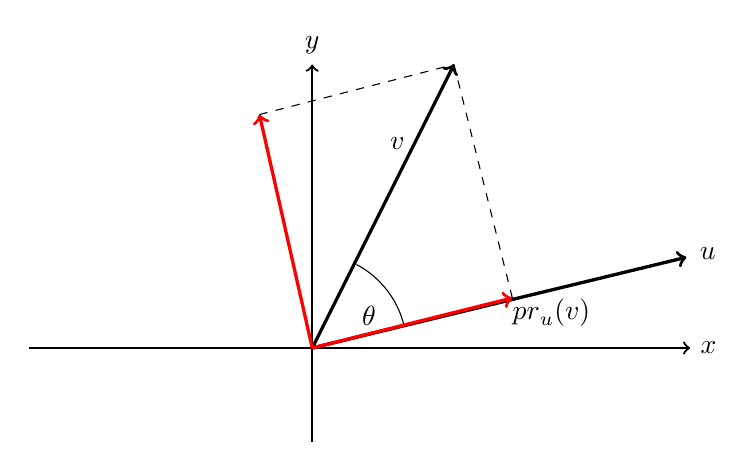
\begin{tikzpicture}[scale=1.2]
                \draw[thick,->] (-3.0,0) -- (4.0,0) node[right] {$x$}; % eje x
                \draw[thick,->] (0,-1) -- (0,3) node[above] {$y$}; % eje y
                %\foreach \x in {-2,...,3}
                %\draw (\x,3pt) -- (\x,-3pt);
                %\foreach \y in {0,...,2}
                %\draw (3pt,\y) -- (-3pt,\y) ;
                % vector u
                %\draw[fill] (3,1) circle [radius=0.05];
                \node [right] at (4,1) {$u$};
                \draw[very thick, ->] (0,0) -- (3.96,0.96);
                % vector v
                %\draw[fill] (1,2) circle [radius=0.05];
                \draw[very thick,->] (0,0) -- (1.5,3);
                \node [above] at (0.9,2) {$v$};
                % flecha punteada de w a v
                \draw [domain=13.5:62] plot ({cos(\x)}, {sin(\x)});
                \node [above] at (0.6,0.13) {$\theta$};
                \draw[->, very thick,red] (0,0) -- (36/17,9/17);
                \node [anchor=north west] at (-0.1+36/17,0.1+9/17) {$\operatorname{pr}_u(v)$};
                \draw[->, very thick,red] (0,0) -- (-9.5/17,42/17);
                % vector v - w
               %+--- \draw[fill] (-2,1) circle [radius=0.05];
                % punteada de v-w  a v
                \draw[dashed] (-9.5/17,42/17) -- (1.5,3);	
                \draw[dashed] (36/17,9/17) -- (1.5,3);	
                
                \end{tikzpicture}
                \caption{Proyección de $v$ en $u$ cuando $||v||=1$.}\label{fig-proyeccion-ort}
            \end{figure}
        
        
            Esto,  además de la interpretación geométrica, lo podemos demostrar algebraicamente:
            \begin{equation*}
            \la v - \frac{\la u,v\ra}{\la u,u\ra} u , u \ra =
            \la v , u \ra  -\frac{\la u,v\ra}{\la u,u\ra}\la u , u \ra =  \la v , u \ra -  \la u , v \ra =0.
            \end{equation*}
            
        \end{observacion}
        
        \begin{proposicion}[Desigualdad de Cauchy-Schwarz]\label{prop-cauchy-schwarz} Sean $u, v\in \R^n$. Entonces 
            $$|\la u, v \ra| \le ||u||||v||.$$
        \end{proposicion}
        \begin{proof} 
            Sea $c = \displaystyle\frac{\la u,v\ra}{\la u,u\ra} = \frac{\la u,v\ra}{||u||^2}$, entonces, por la observación \ref{obs-proyeccion-ort}, tenemos que  $ v-cu$ es ortogonal a $u$. Ahora bien, 
            \begin{equation*}
                v = (v - cu) + cu   
            \end{equation*}
            y  $(v - cu) \perp cu$. Por Pitágoras
            \begin{align*}
            ||v||^2 &= ||v-cu||^2 +||cu||^2  \\
            &=||v-cu||^2 +|c|^2||u||^2.
            \end{align*}
            Como $||v-cu||^2 \ge 0$, tenemos que $|c|^2||u||^2 \le 	||v||^2$ y sacando raíces cuadradas obtenemos
            $$
            |c|||u|| \le ||v|| \Rightarrow \frac{|\la u,v\ra|}{||u||^2}||u|| \le ||v|| \Rightarrow \frac{|\la u,v\ra|}{||u||}\le ||v|| \Rightarrow |\la u,v\ra|\le ||v||||u||.
            $$
        \end{proof}
        
        \begin{teorema}[Desigualdad triangular] Sean $u, v\in \R^n$, entonces 
            $$||u + v|| \le ||u|| + ||v||	$$
        \end{teorema}
        \begin{proof}
            Probar 
            $$
            ||u + v||^2 \le (||u|| + ||v||)^2
            $$
            desarrollando  el lado izquierdo de la desigualdad  como $\la u+v, u+v \ra$ y el lado derecho por el cálculo del binomio al cuadrado. Luego usar la desigualdad de Cauchy-Schwarz.
        \end{proof}
        
        Ahora vamos a demostrar el proceso de ortonormalización de Gram-Schmidt, que consta de  un algoritmo que permite pasar de una base cualquiera $\{v_1,\ldots, v_n\}$ de $\R^n$ a una base ortonormal $\{u_1,\ldots, u_n\}$, con la importante propiedad de que, para $m$ con  $1 \le m \le n$, el subespacio generado por los vectores $\{u_1,\ldots, u_m\}$ es el mismo que el subespacio generado por los vectores $\{v_1,\ldots, v_m\}$.

        
        La idea del proceso es sencillo para dos vectores: sean  $v_1,v_2 \in \R^n$ no  nulos y no proporcionales, vimos en la observación \ref{obs-proyeccion-ort} que  los vectores
        \begin{equation*}
            w_1 = v_1, \quad w_2 = v_2 - \operatorname{pr}_{v_1}(v_2) = v_2 - \frac{\la v_1,v_2\ra}{\la v_1,v_1\ra}v_1
        \end{equation*}
        son ortogonales. Ahora bien, $v_1 = w_1$ y $v_2  = \frac{\la v_1,v_2\ra}{\la v_1,v_1\ra}w_1 + w_2$, luego  $w_1,w_2$ generan el mismo subespacio que $v_1,v_2$. Concluyendo, dados  $v_1,v_2$ dos vectores LI, $w_1,w_2$ son dos vectores ortogonales que generan el mismo subespacio. Para $n >2$ la idea es similar. 
        
  
        
        
        
        \begin{proposicion}[Proceso de ortogonalización de Gram-Schmidt]\index{Gram-Schmidt}
            Sea $\{v_1,\ldots,v_n\}$ una base de $\R^n$. Entonces existe una base ortogonal $\{w_1,\ldots, w_n\}$ tal que el subespacio generado por los vectores $\{w_1,\ldots, w_m\}$ es el mismo que el subespacio generado por $\{v_1,\ldots, v_m\}$ ($1\le m \le n$). Explícitamente, la base es
            \begin{align}
            w_1 &= v_1, \tag{1} \\
            w_2 &= v_2 - \frac{\la v_2,w_1\ra}{\la w_1,w_1\ra}w_1, \tag{2}\\
            w_3 &= v_3 - \frac{\la v_3,w_1\ra}{\la w_1,w_1\ra}w_1- \frac{\la v_3,w_2\ra}{\la w_2,w_2\ra}w_2,\tag{3} \\
            \vdots &\quad \vdots \notag \\
            w_n &= v_n - \frac{\la v_n,w_1\ra}{\la w_1,w_1\ra}w_1- \frac{\la v_n,w_2\ra}{\la w_2,w_2\ra}w_2 - \cdots - \frac{\la v_n,w_{n-1}\ra}{\la w_{n-1},w_{n-1}\ra}w_{n-1}.\tag{$n$}	
            \end{align}
            En forma más breve, para $1 \le i \le n$, 
            \begin{equation}
            w_i = v_i - \sum_{j = 1}^{i-1} \frac{\la v_i,w_{j}\ra}{\la w_{j},w_{j}\ra}w_{j} \tag{$i$}
            \end{equation}
        \end{proposicion} 
        \begin{proof}[Demostración ($*$)]
            
            
            Haremos la demostración por inducción sobre $n$. 
            
            Para $n= 1$ el resultado es trivial.
            
            Supongamos que el resultado valga para $k-1>0$, es decir  $\{w_1,\ldots, w_{k-1}\}$ es ortogonal y 
            $\operatorname{span}(w_1,\ldots, w_{k-1}) = \operatorname{span}(v_1,\ldots, v_{k-1})$. Probemos el resultado para $k$.  Si  $i < k$, 
            \begin{align*}
            \la w_k, w_i \ra &= \la  v_k - \sum_{j = 1}^{k-1} \frac{\la v_k,w_{j}\ra}{\la w_{j},w_{j}\ra}w_{j} , w_i \ra 
            = \la v_k, w_i\ra -  \sum_{j = 1}^{k-1} \frac{\la v_k,w_{j}\ra}{\la w_{j},w_{j}\ra}\la w_{j} , w_i \ra \\
            &=  \la v_k, w_i\ra -  \la v_k, w_i\ra = 0.
            \end{align*}
            Es decir $	\la w_k, w_i \ra =0$ para todo $i < k$. Por consiguiente,  $\{w_1,\ldots, w_{k}\}$ es ortogonal.
            
            Demostremos ahora que $\operatorname{span}\{w_1,\ldots, w_{m}\} = \operatorname{span}\{v_1,\ldots, v_{m}\}$ para $1 \le m \le n$. 
            
            $\operatorname{span}\{w_1,\ldots, w_{m}\} \subset \operatorname{span}\{v_1,\ldots, v_{m}\}$: por la fórmula ($i$) es claro que $w_m$  es combinación lineal de $v_m$ y $w_1,\ldots, w_{m-1}$. Por hipótesis inductiva, los $w_1,\ldots, w_{m-1}$ son combinación lineal de  los $v_1,\ldots, v_{m-1}$,  luego los $w_1,\ldots, w_{m}$ son combinación lineal de los  $v_1,\ldots, v_{m}$.
            
            $\operatorname{span}\{v_1,\ldots, v_{m}\} \subset \operatorname{span}\{w_1,\ldots, w_{m}\}$: Como
            $$
            v_k = w_k + \sum_{j = 1}^{k-1} \frac{\la v_k,w_{j}\ra}{\la w_{j},w_{j}\ra}w_{j},
            $$
            tenemos que 	$\operatorname{span}\{v_1,\ldots, v_{m}\} \subset \operatorname{span}\{w_1,\ldots, w_{m}\}$.
        \end{proof}
        
        

        
        \begin{observacion*} Sea $W$ subespacio de $\R^n$, entonces existe una base ortogonal de $W$. Esto se deduce del proceso de ortogonalización de Gram-Schmidt: sea $v_1,\ldots,v_k$ una base de $W$ y completamos a $v_{1},\ldots,v_n$ una base de $\R^n$. Por Gram-Schmidt obtenemos una BO $w_{1},\ldots,w_n$ tal que el subespacio generado  por $w_{1},\ldots,w_i$ es igual al subespacio generado por $v_{1},\ldots,v_i$ para $1 \le i \le n$. En  particular $W = \la v_{1},\ldots,v_k \ra =  \la w_{1},\ldots,w_k \ra$ y por lo tanto  $w_{1},\ldots,w_k$ es una BON de $W$.
            
        En la práctica, dada una base $v_1,\ldots,v_k$ de $W$,  con los primeros $k$ pasos del proceso de ortogonalización de Gram-Schmidt obtenemos $ w_{1},\ldots,w_k $ una base ortogonal de $W$.
        \end{observacion*}
        
        \begin{ejemplo*}
            Encontrar una base ortogonal del subespacio de $\R^3$ generado por los vectores $(1,2,-1)$ y $(-2,-1,0)$
            \begin{proof}[Solución] Por Gram-Schmidt:
                \begin{align*}
                w_1 &= (1,2,-1),  \\
                w_2 &= (-2,-1,0) - \frac{\la (-2,-1,0),w_1\ra}{\la w_1,w_1\ra}w_1,
                \end{align*}
                es una base ortogonal de $W$. Calculemos 
                \begin{align*}
                    w_2  &= (-2,-1,0) - \frac{\la (-2,-1,0),(1,2,-1)\ra}{\la(1,2,-1),(1,2,-1)\ra}(1,2,-1)\\
                    &= (-2,-1,0) - \frac{-4}{6}(1,2,-1) \\
                    &= (-2,-1,0) - (\frac{-2}{3},\frac{-4}{3},\frac{2}{3}) \\
                    &= (\frac{-4}{3},\frac{1}{3},\frac{-2}{3}).
                \end{align*}
                Para simplificar, multiplicamos a $w_2$ por $3$ y obtenemos que
                \begin{equation*}
                    (1,2,-1), (-4,1,-2)
                \end{equation*} 
                es una BO de $W$. 
                
            \end{proof}  
        \end{ejemplo*}
        

        
        \begin{definicion}  Sean $U, W$ subespacios de $\R^n$. Diremos que \textit{$U$ es ortogonal a $W$} y denotaremos $U \perp W$ si  para todo $u \in U$ y para todo $w \in W$ tenemos que $ \la u,w\ra =0$. 
            
            Si $X$ es subconjunto de $\R^n$,  definimos 
            $$
            X^\perp := \{u \in \R^n: \la u,x\ra = 0, \forall\, x \in X\} = \{u \in \R^n: \la u,X\ra = 0\}.
            $$ 
        \end{definicion}
        
        \begin{proposicion}
            Sea  $X \subset \R^n$, entonces $X^\perp$  es un subespacio de $\R^n$.
        \end{proposicion}
        \begin{proof}
            Debemos probar que si $u,v \in X^\perp$ y $c \in \R$,  entonces $cu+v \in X^\perp$,  es decir que para todo $x \in X$,  se cumple que  $\la cu+v,x\ra=0$. Ahora bien,
            $$
            \la cu+v,x\ra= c\la u,x\ra +\la v,x\ra= 0.
            $$
        \end{proof}
        
        \begin{definicion}
            Sea $\R^n$ espacio vectorial con producto interno $\la \;,\;\ra$ y sea $X$ subconjunto de $\R^n$. Diremos que $X^\perp$ es el  \textit{subespacio  ortogonal a $X$ en $\R^n$}.   
        \end{definicion}
        
    
    \end{section}


    
	\begin{section}{Suma directa de subespacios y proyecciones  (*)}
		
		En esta sección se define la descomposición de un espacio vectorial como suma directa de dos subespacios. Se muestra que esa descomposición equivale a a definir un operador idempotente en el espacio, al cual llamaremos \textit{proyección}.
		
		\medskip
		
		Si  $V_1$, $V_2$, $W$  dos subespacios del espacio vectorial $V$,  entonces sabemos que 
		\begin{equation*}
		V_1 + V_2 = \{v_1+v_2: v_1 \in V_1, v_2 \in V_2\}, \qquad V_1 \cap V_2 = \{v: v \in V_1 \text{ y } v \in V_2 \}
		\end{equation*}
		son subespacios vectoriales. 
		
		\begin{definicion} Sean $V_1$, $V_2$, $W$  subespacios vectoriales del espacio vectorial $V$, entonces 
			\begin{equation*}
			W = V_1 \oplus V_2
			\end{equation*}
			es la \textit{suma directa}\index{suma directa} de $V_1$ y $V_2$ si $V_1 + V_2 = W$ y $V_1 \cap V_2 = 0$. 
		\end{definicion}
		
		\begin{proposicion}
			Sea $V$  espacio vectorial y $V_1$, $V_2$ subespacios vectoriales de $V$. Entonces, $V = V_1 \oplus V_2$ si y sólo si para todo vector $v \in V$ existe únicos  $v_1\in V_1, v_2 \in V_2$ tal que $v = v_1 + v_2$. 
		\end{proposicion}
		\begin{proof} {\,${}^{}$}
			\begin{enumerate}
				\item[$(\Rightarrow)$] Sea $v \in V$,  como $V = V_1 + V_2$, existen $v_1\in V_1, v_2 \in V_2$ tal que $v = v_1 + v_2$. Veamos que $v_1$ y $v_2$ son  únicos. Sean $v'_1\in V_1, v'_2 \in V_2$ tal que $v = v'_1 + v'_2$. Por lo tanto $v_1 + v_2 =  v'_1 + v'_2$. Haciendo pasajes de término obtenemos 
				$$
				v_1 -v_1' = v_2' - v_2.
				$$
				Sea  $v_0=v_1 -v_1' = v_2' - v_2$. Ahora bien, $v_1 -v_1' \in V_1$, por lo tanto $v_0= v_1 -v_1'  \in V_1$. Análogamente,  $v_2' -v_2 \in V_2$, por lo tanto $v_0= v_2' -v_2  \in V_2$. Es decir, $v_0 \in V_1 \cap V_2 = 0$, luego $v_0 =0$, por lo tanto $v_1 = v'_1$ y $v_2 = v'_2$. 
				\item[$(\Leftarrow)$] Es claro que $V = V_1 + V_2$. Probemos que $V_1 \cap V_2 = 0$. Sea $v \in V_1 \cap V_2$. Por hipótesis, existe únicos $v_1\in V_1, v_2 \in V_2$ tal que $v = v_1 + v_2$.
				Podemos escribir  entonces
				$$
				\begin{array}{rcllll}
				v &=& v_1 + v_2,& \quad &v_1\in V_1,& v_2 \in V_2 \\
				v &=& v + 0,& \quad &v\in V_1, &0 \in V_2 \\
				v &=& 0 + v& \quad &0\in V_1, &v \in V_2. 
				\end{array}
				$$
				Por la unicidad, resulta que $v_1 = v= 0$ y $v_2 = 0 =v$, es decir $v =0$.
			\end{enumerate}	
			
		\end{proof}
		\medskip 
		
		\begin{proposicion} Sea $V$  espacio vectorial de dimensión finita y sean $V_1$, $V_2$ dos subespacios de  $V$ tal que $V = V_1 \oplus V_2$. Sea $\mathcal{B}_1$ base de $V_1$ y $\mathcal{B}_2$ base de $V_2$, entonces $\mathcal{B} = \mathcal{B}_1 \cup \mathcal{B}_2$ es base de $V$.
		\end{proposicion}
		\begin{proof}
			Sea $\mathcal{B}_1 = \{u_1,\ldots,u_r \}$ y $\mathcal{B}_2 = \{u_{r+1},\ldots,u_{r+s} \}$, debemos ver entonces que el conjunto  $\mathcal{B} = \{u_{1},\ldots,u_{r+s} \}$  genera todo el espacio y es LI.
            \vskip .2cm
			\noindent \textit{$\mathcal{B}$ genera $V$.}  Sea $v \in V$, como $V_1 + V_2 = V$, existen $v_1 \in V_1$ y  $v_2 \in V_2$ tales que $v = v_1 + v_2$. Como  $\mathcal{B}_1$ es base de $V_1$, tenemos que $v_1 = a_1u_1+\cdots+a_ru_r$, análogamente
			$v_2 = a_{r+1}u_{r+1}+\cdots+a_{r+s}u_{r+s}$ y por lo tanto $v = a_{1}u_{1}+\cdots+a_{r+s}u_{r+s}$. Es decir  $\mathcal{B}$ genera $V$.
			\vskip .2cm
			\noindent \textit{$\mathcal{B}$ es LI.} Si $a_1u_1+\cdots+a_ru_r + a_{r+1}u_{r+1}+\cdots+a_{r+s}u_{r+s} = 0$, entonces 
			$$a_1u_1+\cdots+a_ru_r = - a_{r+1}u_{r+1}-\cdots-a_{r+s}u_{r+s}.$$ Ahora bien, el termino de la izquierda en la última igualdad pertenece a $V_1$, mientras que el de a derecha pertenece a $V_2$. Como $V_1 \cap V_2 = 0$, tenemos que
			$$a_1u_1+\cdots+a_ru_r = 0 = - a_{r+1}u_{r+1}-\cdots-a_{r+s}u_{r+s}.$$
			Como $\mathcal{B}_1$ es base de $V_1$, $a_1 = \cdots = a_r = 0$ y como $\mathcal{B}_1$ es base de $V_1$, $a_{r+1} = \cdots = a_{r+s} =0$. Es decir $\mathcal{B}$ es LI.	
		\end{proof}
		
		\begin{corolario}
			Sea $V$  espacio vectorial de dimensión finita y sean $V_1$, $V_2$ dos subespacios de  $V$ tal que $V = V_1 \oplus V_2$.  Entonces $\dim(V) = \dim(V_1) + \dim(V_2)$.
		\end{corolario}
		\begin{proof}
			Sea $\mathcal{B}_1 = \{u_1,\ldots,u_r \}$ base de $V_1$ y $\mathcal{B}_2 = \{u_{r+1},\ldots,u_{r+s} \}$ base de $V_2$. Por la proposición anterior, $\mathcal{B} = \{u_{1},\ldots,u_{r+s} \}$ es base de $V$. Luego   $\dim(V) = r +s = \dim(V_1) + \dim(V_2)$.
		\end{proof}
		
		Se puede generalizar la noción de suma directa a varios subespacios. 
		
		\begin{definicion} Sean $V_1,\ldots,V_k$, $W$  subespacios vectoriales de un espacio vectorial $V$, entonces 
			$$
			W = V_1 \oplus V_2 \oplus \cdots \oplus V_k 
			$$ 
			si $V_1 + V_2 + \cdots +V_k= W$ y $V_j \cap (\sum_{i \ne j}V_i) = 0$. En  este caso  diremos que  $W$ es \textit{suma directa} de $V_1,\ldots,V_k$.
		\end{definicion}
		
		Esta definición se reduce  a la de suma directa de dos subespacios cuando $k=2$.
		
		Observar que si definimos $W_j = \sum_{i \ne j}V_i$ ($j=1,\ldots,k$) entonces, 
		$$W = V_1 \oplus V_2 \oplus \cdots \oplus V_k \;\text{ si y sólo si }\;W = V_j \oplus W_j\text{ \; }(j=1,\ldots,k).
		$$
		
        \begin{definicion} Sea $W$  un subespacio vectorial de un espacio vectorial $V$. Entonces un \textit{complemento de $W$} es un subespacio $U$ de $V$ tal que $V=W\oplus U$. 
		\end{definicion}
		
		\begin{proposicion} Sea $V$  espacio vectorial de dimensión finita y sea $W$ un subespacio de  $V$. Sean $\mathcal{B}_W$ una base de $W$ y $\mathcal{B}_V$ una base de $V$ tal que $\mathcal{B}_W\subset \mathcal{B}_V$. 
			
			Sea 
			\[
			\mathcal{B}'=\mathcal{B}_V -\mathcal{B}_W=\{b\in\mathcal{B}_V \text{ tales que } b\notin\mathcal{B}_W \}.
			\]  
			Entonces $U=\langle 	\mathcal{B}'\rangle$ es un complemento de $W$ y $\mathcal{B}'$ es una base de $U$.
		\end{proposicion}
		\begin{proof}
			Sea $\mathcal{B}_W = \{u_1,\ldots,u_r \}$ y $\mathcal{B}_V = \{u_1,\ldots,u_r, u_{r+1},\ldots,u_{r+s}\}$. Así, 	$\mathcal{B}'=\{u_{r+1},\ldots,u_{r+s} \}$. Como este conjunto es LI, entonces es una base del espacio $U=\langle 	\mathcal{B}'\rangle$ que genera. Por otro lado, como $\mathcal{B}_V$ es base de $V$, entonces todo vector $v\in V$ puede escribirse como
			\[
			v=a_1u_1+\cdots+a_ru_r + a_{r+1}u_{r+1}+\cdots+a_{r+s}u_{r+s},
			\]
			para algunos $a_1,\dots a_{r+s}\in \K$.				
			Ahora, definimos $v_W=a_1u_1+\cdots+a_ru_r$ y $v_U=a_{r+1}u_{r+1}+\cdots+a_{r+s}u_{r+s}$, de manera tal que  $v_W\in W$, $v_U\in U$ y $v=v_W+v_U$.
			
			Finalmente, si $v\in W\cap U$, entonces existen $a_1,\dots a_{r+s}\in \K$ tales que 
			\[
			v=a_1u_1+\cdots+a_ru_r = a_{r+1}u_{r+1}+\cdots+a_{r+s}u_{r+s}.
			\]
			Pero esto determina que $\mathcal{B}_V$ es LI (es una base). Luego, $W\cap U=\{0\}$ y por lo tanto $V=W\oplus U$.
		\end{proof}
		
		La noción de suma directa está ligada a la noción de proyección.
		
        \begin{definicion} Sea $V = W \oplus U$. Definimos el operador lineal $P: V \to V$ por  $$P(w+u) = w,$$ con $w \in W$, $u\in U$. En este caso, diremos que $P$ es la \textit{proyección a $W$ paralela a $U$}. Si $V$  es un espacio con producto interno y  $W \perp U$, diremos que $P$ es la \textit{proyección ortogonal sobre $W$}. 
		\end{definicion}
		
		Observar que $P$ está bien definida y que $P_{|W} = Id_{|W}$,  $P_{|U} = 0$. Observar también que si $P$  es una proyección ortogonal,  entonces $U = W^\perp$, luego $U$  está determinado por $W$. . 
		
		\medskip 
		
		\begin{proposicion}\label{matriz-proy}
			Sea $P: V \to V$ una proyección, entonces existe una base $\mathcal{B}$ tal que 
			$$
			[P]_{\mathcal{B}} = diag(1,\ldots,1,0,\ldots,0).
			$$
			(una  matriz diagonal con la diagonal compuesta de  $1$'s  y a continuación $0$'s).
		\end{proposicion}
		\begin{proof}
			Sean $V_1,V_2$ subespacios de $V$ tal que   $P$ es la {proyección a $V_1$ paralela a $V_2$}. Sea $\{v_1,\ldots,v_m\}$ una base de $V_1$ y completamos con $\{v_{m+1},\ldots,v_n\}$, vectores en $V_2$, a una base de $V$. Sea $\mathcal{B}= \{v_1,\ldots,v_n\}$. Como  $P_{|V_1} = Id_{|V_1}$ y  $P_{|V_2} = 0$, es claro que $
			[P]_{\mathcal{B}} = diag(1,\ldots,1,0,\ldots,0)
			$, donde la cantidad de $1$'s es  $m$  y la cantidad de $0$'s es $n-m$.
		\end{proof}
		
		\medskip
		
		\begin{definicion} Sea $V$ espacio vectorial de dimensión finita. $P:V \to V$ una aplicación lineal. Diremos que $P$ es \textit{idempotente} si $P\circ P = P$. Denotemos $P \circ P = P^2$.
		\end{definicion}
		
		
		
		
		\begin{proposicion}\label{proy->idem}
			Sea $P: V \to V$ una proyección a  $W$ paralela a  $U$, entonces $P^2 = P$.
		\end{proposicion}
		\begin{proof}
			Como $P$ proyecta a  $W$ de forma paralela a  $U$, entonces para $w \in W, u \in U$ tenemos  $P(w+u) = w$, por lo tanto  $P^2(w+u) = P(w) = w= P(w+u)$.
		\end{proof}
		
		\begin{teorema}\label{idem->proy}
			Sea $P: V \to V$ un operador lineal. Si $P^2 = P$  entonces
			$$
			V = \nu(P) \oplus \im(P).
			$$
			Además, $P$ es la proyección  a $\im(P)$ paralela a $\nu(P)$.
		\end{teorema}
		\begin{proof} Veamos primero que $\nu(P) \cap \im(P)= 0$. Sea $v \in \nu(P) \cap \im(P)$. Como $v \in \im(P)$, entonces $v = P(w)$, luego   $P(v) = P^2(w) =P(w) = v$. Ahora bien, como $v\in  \nu(P)$, entonces $P(v)=0$. Es decir, si  $v \in\nu(P) \cap \im(P)$, entonces  $v= P(v)=0$. 
			
			Observar que $v = (v -P(v)) + P(v)$ y que $v -P(v)\in \nu(P)$ y $P(v) \in \im(P)$. Luego $v \in \nu(P) + \im(P)$. Como $v \in V$ es arbitrario,  tenemos que $V= \nu(P) + \im(P)$
		\end{proof}

		\begin{teorema} 
			Sea $V$ espacio vectorial de dimensión finita y $P:V \to V$ una aplicación lineal. Entonces, $P$ es una proyección a $W$ paralela a  $U$ si y sólo si $P^2 = P$ y $W= \im(P)$, $U = \nu(P)$. 
		\end{teorema}
		\begin{proof} ($\Rightarrow$) es proposición \ref{proy->idem}. ($\Leftarrow$) es teorema \ref{idem->proy}.
        \end{proof}
		
	\end{section}


    \begin{section}{La adjunta de una transformaci\'on lineal (*)}\label{seccion-adjunta-de-una-transformacion-lineal} Mostraremos en esta sección como el producto interno nos permite asociar a cada transformación lineal $T: V \to W$ una nueva transformación  lineal $T^*: W \to V$ llamada la adjunta de $T$. 
	
        \begin{teorema}
            Sean $V, W$ espacios vectoriales de dimensión finita y con producto interno $\la \;,\;\ra$ y $\la \;,\;\ra$ respectivamente (se denotan igual). Sea $T: V \to W$ lineal, entonces existe una única $T^*: W \to V$ que cumple
            \begin{equation}\label{eq-adjunta}
            \la Tv,w\ra = \la v,T^*w\ra,
            \end{equation}  
            para $v\in V$, $w \in W$ (el producto de la izquierda es en $W$ y el de la derecha en $V$).
        \end{teorema}
        \begin{proof}
        Sea $\{v_1,\ldots,v_n\}$ una BON de $V$ y $\{w_1,\ldots,w_m\}$ una BON de $W$, observemos que la coordenada $j$ (en $V$) de $T^*w_i$ debe cumplir
        \begin{equation}\label{eq-transp}
            \la T^*w_i,v_j\ra = 	\la w_i,Tv_j\ra.
        \end{equation}
        Por lo tanto,  definimos
        \begin{equation*}
            T^*(w_i) = \sum_{j=1}^{n} \la w_i,Tv_j\ra v_j,
        \end{equation*}
        y extendemos linealmente a una transformación lineal $T^*: W \to V$. Claramente $T^*$   está bien definida y es lineal (por definición).  La unicidad está garantizada por la ecuación \eqref{eq-transp}.  
        
        Finalmente,  debemos comprobar que se verifica la ecuación \eqref{eq-adjunta}: sean  $w \in W$ y $v \in V$, entonces $w = \sum_{i=1}^{m} \la w_i,w\ra w_i$ y $v = \sum_{j=1}^{n} \la v_j,v\ra v_j$. Reemplazando en  la ecuación \eqref{eq-adjunta} $w$ y $v$ por su desarrollo en las bases se obtiene la igualdad. Para el lector curioso, a continuación desarrollamos la demostración:
        \begin{align*}
            \la v,T^*w\ra &= 	\la v, T^*(\sum_{i=1}^{m} \la w_i,w\ra w_i) \ra\\
             &= \la v, \sum_{i=1}^{m} \la w_i,w\ra T^*(w_i) \ra\\
             &=	\sum_{i=1}^{m} \la w_i,w\ra\la v,  T^*(w_i) \ra\\
             &=\sum_{i=1}^{m} \la w_i,w\ra\la v,  \sum_{j=1}^{n} \la w_i,Tv_j\ra v_j\ra\\
             &=\sum_{i=1}^{m} \la w_i,w\ra \sum_{j=1}^{n} \la w_i,Tv_j\ra\la v,  v_j\ra.
        \end{align*}
        Por otro lado, como $v = \sum_{j=1}^{n} \la v_j,v\ra v_j$, entonces
        \begin{equation*}
            \sum_{j=1}^{n} \la w_i,Tv_j\ra\la v,  v_j\ra = \sum_{j=1}^{n} \la w_i,\la v,  v_j\ra Tv_j\ra = \la w_i, T (\sum_{j=1}^{n}\la v,  v_j\ra v_j)\ra = \la w_i, T v\ra, 
        \end{equation*}
        por lo tanto 
        \begin{equation*}
            \la v,T^*w\ra = \sum_{i=1}^{m} \la w_i,w\ra \la w_i, T v\ra =  \la\sum_{i=1}^{m} \la w_i,w\ra w_i, T v\ra = \la w, T v\ra
        \end{equation*}
        \end{proof}
        
        \begin{definicion}
            Sean $V, W$ espacios vectoriales de dimensión finita y con producto interno $\la \;,\;\ra$ y $\la \;,\;\ra$ respectivamente. Sea $T: V \to W$ lineal, entonces a la única $T^*: W \to V$ que cumple
            \begin{equation}\label{eq-adjunta}
            \la Tv,w\ra = \la v,T^*w\ra,
            \end{equation}  
            para $v\in V$, $w \in W$ se la denomina la \textit{adjunta de $T$}.\index{adjunta de una transformación lineal}
        \end{definicion}
        
        \begin{observacion*} El caso más interesante, y que pasaremos a estudiar ahora, es cuando $T: V \to V$, es decir cuando el espacio de llegada y  de partida es el mismo, y por lo tanto también $T^*: V \to V$. 
        \end{observacion*}
        
        
        \begin{ejemplo*}\label{ejemplo4.10}
            Sea $T: \R^3 \to \R^3$ la transformación lineal $T(x,y,z) = (3x +y, 2x -y+ 3z, x)$. Calcular $T^*$ y la matriz de $T$ y $T^*$ en la base canónica.  
        \end{ejemplo*}
        \begin{proof}[Solución 1] 
            La observación principal para hacer el cálculo de $T^*$ es que dada cualquier transformación lineal $S$, tenemos que 
            $$
            \la e_i, S(v)\ra  = t_i \Leftrightarrow S(v) = (t_1,\ldots,t_n). 
            $$ 
            Aplicado a este caso,
            \begin{align*}
            \la e_1, T^*(x,y,z)\ra  &= \la  T(e_1),(x,y,z)\ra =    \la (3,2,1),(x,y,z)\ra = 3x+2y+z \\
            \la e_2, T^*(x,y,z)\ra  &= \la  T(e_2),(x,y,z)\ra =    \la (1,-1,0),(x,y,z)\ra = x-y \\
            \la e_3, T^*(x,y,z)\ra  &= \la  T(e_3),(x,y,z)\ra =    \la (0,3,0),(x,y,z)\ra = 3y. \\
            \end{align*}
            Por lo tanto
            $$
            T^*(x,y,z) = (3x+2y+z,x-y,3y).
            $$
            La matriz de $T$ en la base canónica es 
            $$
            \left[\begin{matrix}
            3&1&0\\2&-1&3\\1&0&0.
            \end{matrix}
            \right]
            $$
            y la matriz de $T^*$ en la base canónica es
            $$
            \left[\begin{matrix}
            3&2&1\\1&-1&0\\0&3&0.
            \end{matrix}
            \right]
            $$
        \end{proof}
        
        
        Observemos que en el ejemplo anterior la matriz de la adjunta es la transpuesta de la matriz de la transformación original. Veremos ahora, que este es un resultado general. 
        
        \begin{teorema}\label{matrizadjunta}
            Sea $V$ espacio vectorial de dimensión finita con producto interno $\la \;,\;\ra$ y sea  $\mathcal U = \{u_1, \ldots , u_n\}$ una BON de $V$. Sea $T: V \to V$ una transformación lineal y $A$ la matriz de $T$ en  la base $\mathcal U$,  es decir $[T]_{\mathcal U} = A$.
            
            Entonces, $[T^*]_{\mathcal U} = A^\t$, es decir, la matriz de $T^*$ en la base $\mathcal U$ es la transpuesta de $A$. 
        \end{teorema}
        \begin{proof}
            Observemos  que como $T(u_j) = \sum_i a_{ij}u_i$, entonces 
            $$
            \la Tu_j,u_i\ra = a_{ij}.
            $$
            Luego 
            $$
            a_{ij} = \la Tu_j,u_i\ra = \la u_j,T^*u_i\ra.
            $$
            Es decir  que $T^*(u_i) = \sum_j a_{ij}$. Es decir $[T^*]_{\mathcal U} = A^\t$.
        \end{proof}
        
        
    
        
        \begin{ejemplo*} Resolveremos nuevamente, en forma más sencilla, el ejemplo anterior.
        \end{ejemplo*}
        \begin{proof}[Solución 2]
            Como $T(x,y,z) = (3x +y, 2x -y+ 3z, x)$, la matriz de $T$ en la base canónica es 
            $$
            \left[\begin{matrix}
            3&1&0\\2&-1&3\\1&0&0.
            \end{matrix}
            \right].
            $$
            Por lo tanto, por teorema  \ref{matrizadjunta}, la matriz de $T^*$ en la base canónica es
            $$
            \left[\begin{matrix}
            3&2&1\\1&-1&0\\0&3&0.
            \end{matrix}
            \right].
            $$
            Luego $T^*(x,y,z) = (3x+2y+z,x-y,3y)$.
        \end{proof}

    
        
        \begin{proposicion}\label{adjprop}
            Sean $V$ espacio vectorial de dimensión finita con producto interno $\la \;,\;\ra$ y $T,S:V \to V$ transformaciones lineales. Entonces
            \begin{enumerate}
                \item\label{adj0} $Id^* = Id$.
                \item\label{adj1} Si $c \in \R$, entonces $(cR)^* = cR^*$.
                \item\label{adj2} $(R+S)^* = R^* + S^*$.
                \item\label{adj3} $(RS)^* = S^*R^*$.
                \item\label{adj4} $R^{**} = R$.
            \end{enumerate} 
        \end{proposicion}
        \begin{proof}
            \ref{adj0} Es trivial.
            
            \ref{adj1} Por definición de adjunta $(cR)^*$ es la única transformación lineal tal que
            $$
            \la cR(v),w\ra = \la v,(cR)^*(w)\ra, \quad \forall v,w \in V.
            $$
            Ahora bien
            $$
            \la v,cR^*(w)\ra = c\la v,R^*(w)\ra = c\la R(v),w\ra =  \la cR(v),w\ra. 
            $$
            Es decir $(cR)^* = cR^*$.
            
            \ref{adj2} Como en el caso anterior, debemos demostrar que  $R^* + S^*$ es la única transformación lineal tal que
            $$ 
            \la (R+S)(v),w\ra = \la v,(R^* + S^*)(w)\ra, \quad \forall v,w \in V.
            $$
            Ahora bien,
            \begin{align*}
            \la v,(R^* + S^*)(w)\ra &= \la v,R^*(w) + S^*(w)\ra =  \la v,R^*(w) \ra+\la v, S^*(w)\ra \\
            &=  \la R(v),w \ra+\la S(v), w\ra =  \la R(v) + S(v), w\ra \\
            &=  \la (R+S)(v), w\ra .
            \end{align*}

            \ref{adj3} 
            \begin{align*}
            \la v,(S^*R^*)(w)\ra &= \la v, S^*(R^*(w))\ra =  \la S(v),R^*(w) \ra \\
            &=  \la R(S(v)),w \ra =  \la (RS)(v), w\ra .
            \end{align*}
            Por lo tanto  $(RS)^* = S^*R^*$.
            
            \ref{adj4} Por definición de adjunta de $R^*$, tenemos que $ (R^*)^*=R^{**}$  es la única transformación lineal tal que 
            $$
            \la R^*(v), w\ra = \la v, R^{**}(w)\ra  , \; \forall\, v,w \in V.
            $$ 
            Ahora bien, por la definición de adjunta de $R$ sabemos que 
            $$
            \la R^*(v), w\ra = \la v, R(w)\ra , \; \forall\, v,w \in V.
            $$ 
            Luego $R = R^{**}$.
            
        \end{proof}
        
        
        \begin{teorema}\label{rel-adj-ort}
            Sea $T: V \to W$ una transformación lineal entre espacios vectoriales de dimensión finita con producto interno. Entonces,
            \begin{enumerate}
                \item\label{itm-nut*-imtp} $\nu(T^*) = \im(T)^\perp$,
                \item\label{itm-imt*-nutp} $\im(T^*) = \nu(T)^\perp$,
                \item\label{itm-nut-imt*p} $\nu(T) = \im(T^*)^\perp$,
                \item\label{itm-imt-nut*p} $\im(T) = \nu(T^*)^\perp$.
            \end{enumerate}
        \end{teorema}
       
        \begin{proof}
            La primera afirmación es la que requiera más trabajo, pues las otras se deducen fácilmente de la primera y del hecho que $T^{**} = T$ y $U^{\perp\perp} = U$. 

          \ref{itm-nut*-imtp}
            \begin{align*}
            w \in  \nu(T^*) &\Leftrightarrow T^*(w) =0 \\&\Leftrightarrow \la v, T^*(w) \ra = 0,\; \forall\, v\in V  \\&\Leftrightarrow \la T(v), w \ra = 0,\; \forall\, v\in V\\&\Leftrightarrow  w \in \im(T)^\perp.
            \end{align*}

           \ref{itm-imt*-nutp}
            \begin{align*}
                \im(T^*) = (\im(T^*)^{\perp})^{\perp} \stackrel{\ref{itm-nut*-imtp}}{=}    \nu(T^{**})^{\perp} = \nu(T)^{\perp}.
            \end{align*}

          \ref{itm-nut-imt*p}
            \begin{align*}
                \nu(T) = \nu(T^{**}) \stackrel{\ref{itm-nut*-imtp}}{=}  \im(T^*)^\perp.
            \end{align*}

           \ref{itm-imt-nut*p}
            \begin{align*}
                \im(T) = \im(T)^{\perp\perp}  \stackrel{\ref{itm-nut*-imtp}}{=}  \nu(T^*)^\perp.
            \end{align*}
        \end{proof}
        
        ${}^{}$

        
    \end{section}



    \begin{section}{Operadores autoadjuntos (*)}\label{secccion-operadores-autoadjuntos}

        En esta sección todos los espacios vectoriales serán sobre $\R$ y de dimensión finita. 

        Generalizaremos ahora el concepto de matriz simétrica. 
        
        \begin{definicion}
            Sea $V$ un espacio vectorial con producto interno y $T: V \to V$ una transformación lineal. Diremos que $T$ es una \textit{transformación lineal autoadjunta}\index{transformación lineal autoadjunta} si $T^* = T$. En  ese caso, también suele decirse que $T$ es un \textit{operador lineal autoadjunto}.\index{operador lineal!autoadjunto}
        \end{definicion}
        
        Claramente, en $\R^n$ con el producto interno canónico,  la multiplicación a izquierda de un vector columna por una matriz simétrica es un operador autoadjunto.  
        
        Del  teorema \ref{matrizadjunta} (y un  poco más) se deduce el siguiente resultado.
        
        \begin{proposicion}\label{auto-impl-sim}
            Sea $V$ un espacio vectorial con producto interno y $T: V \to V$ una transformación lineal. Entonces $T$ es un operador lineal autoadjunto si y sólo si para cualquier $\mathcal{U}$ BON de $V$, la matriz de $T$ en la base $\mathcal{U}$  es simétrica.
        \end{proposicion}
        \begin{proof}
            ($\Rightarrow$) Por teorema \ref{matrizadjunta}, si $A$ es la matriz de $T$, entonces  la  matriz de $T^*$ es $A^\t$. Como $T=T^*$, entonces $A = A^\t$.
            
            ($\Leftarrow$) Por hipótesis, $[T]_\mathcal{U} =[T]_\mathcal{U}^\t $. Pero por el teorema \ref{matrizadjunta}, tenemos que  $[T^*]_\mathcal{U} =[T]_\mathcal{U}^\t$. Por lo tanto $[T^*]_\mathcal{U} = [T]_\mathcal{U}$, lo cual implica que  $T= T^*$.
        \end{proof}
        
        \begin{ejemplo}\label{poautoadjunto} Sea $P:V \to V$ una proyección ortogonal,  entonces $P$ es un operador  autoadjunto. 
            
            Veamos que es así: sea $W\subset V$, tal que $P$ proyecta ortogonalmente a $W$,  es decir $V = W \oplus W^\perp$, con $P(w) = w$, $w \in W$ y $P(w')= 0$, $w' \in W^\perp$. 
            
            Entonces si $v_1,v_2 \in V$, tenemos que $v_1 = w_1 + w'_1,  v_2 = w_2 + w'_2$ con $w_1,w_2 \in W$, $w'_1,w'_2 \in W^\perp$. Luego
            $$
            \la P(v_1),v_2 \ra = \la w_1, w_2+w'_2 \ra = \la w_1,w_2\ra = \la w_1, P(v_2) \ra = \la v_1, P(v_2) \ra. 
            $$
        \end{ejemplo}
        
        
        \begin{proposicion}
            Sea $V$ un espacio vectorial con producto interno. Entonces, el  conjunto de operadores lineales autoadjuntos es un espacio vectorial.  
        \end{proposicion}
        \begin{proof}
            El resultado se deduce fácilmente de  la proposición  \ref{adjprop} \ref{adj1} y   \ref{adj2}.
        \end{proof}
        
        \begin{proposicion} Sean $S$ y $T$ dos operadores lineales autoadjuntos. Entonces, $ST$  es autoadjunto si y sólo  si $S$ y $T$ conmutan. 
        \end{proposicion}
        \begin{proof}
            ($\Rightarrow$) Como $ST$ es autoadjunto, tenemos que $ST = (ST)^*$. Por proposición \ref{adjprop}\,\ref{adj3} tenemos que  $(ST)^* = T^*S^*$, y  como $S,T$ son autoadjuntos $T^*S^* = TS$. 
            Reconstruyendo las igualdades tenemos
            $$
            ST = (ST)^* = T^*S^*= TS,
            $$
            es decir, $S$ y $T$ conmutan.
            
            ($\Leftarrow$)  
            $$
            (ST)^* = T^*S^* = TS = ST.
            $$
        \end{proof}
        
        
        \begin{ejemplo*}
            Sean $T,S: \R^2 \to R^2$ operadores lineales definidos
            $$
            T(x,y) = (x,2y),\quad S(x,y) = (y,x).
            $$
            Calculemos $T^*$ y $S^*$. $T^*$ debe satisfacer  que 
            \begin{align*}
                \la e_1, T^*(x,y)\ra &= \la T(e_1),(x,y) \ra = \la e_1, (x,y) \ra = x, \\
                \la e_2, T^*(x,y)\ra &= \la T(e_2),(x,y) \ra = \la 2e_2, (x,y) \ra = 2y.
            \end{align*}
            Es decir, $T^* = T$. Análogamente, se muestra que $S^* = S$. Ahora bien
            \begin{align*}
            \la e_1, (TS)^*(x,y)\ra &= \la TS(e_1),(x,y) \ra = \la T(e_2), (x,y) \ra = \la 2e_2, (x,y) \ra = 2y, \\
            \la e_2, (TS)^*(x,y)\ra &= \la TS(e_2),(x,y) \ra = \la T(e_1), (x,y) \ra = \la e_1, (x,y) \ra = x.
            \end{align*}
            Es decir $(TS)^*(x,y) = (2y,x)$. Por otro lado,  $TS(x,y) = T(y,x) = (y,2x)$. Luego $(TS)^* \ne TS$, es decir $TS$ no es autoadjunto. 
            
            Esto ocurre pues, $TS(x,y) = (y,2x)$ es distinto a  $ST(x,y) = S(x,2y)= (2y,x)$. Es decir, $S$ y $T$ no conmutan.
        \end{ejemplo*}

        
        \begin{ejemplo*}
            En el ejemplo \ref{poautoadjunto} vimos que si  $P$ es una proyección ortogonal, entonces es  operador autoadjunto. Veamos ahora que es diagonalizable: sea $P$ la proyección ortogonal a $W$, y tomemos $\mathcal{U}_0 = \{u_1,\ldots,u_k\}$ una base de $W$ y  $\mathcal{U}_1 = \{u_{k+1},\ldots,u_n\}$ una base de $W^\perp$, luego $\mathcal{U} = \{u_1,\ldots,u_n\}$ es una base de $V$ con la siguiente particularidad
            $$
            P(u_i) = u_i,\quad 1 \le i \le k, \qquad P(u_i) = 0,\quad k+1 \le i \le n.
            $$
            Luego, la base $\mathcal{U}$ consta de autovectores, de los  cuales los primeros $k$ tienen autovalor $1$ y los siguientes tienen autovalor $0$.
        \end{ejemplo*}
        
                
        Veremos ahora la demostración completa de que un operador autoadjunto es diagonalizable, es decir que hay una base de autovectores del operador. 

        \begin{proposicion}
                Sea $V$ un espacio vectorial con producto interno y $T: V \to V$ una transformación lineal. Sea $W$ un subespacio de $V$ invariante por $T$. Entonces $W^\perp$ es invariante por $T^*$.
        \end{proposicion}
        \begin{proof}
            Debemos ver que $T^*(W^\perp) \subset W^\perp$, es decir que $\la T^*(W^\perp) , W \ra = 0$. Pero,
            $$
            \la T^*(W^\perp) , W \ra = \la W^\perp, T(W) \ra \subseteq  \la W^\perp, W \ra =0.
            $$  
        \end{proof}
        
        De lo cual se deduce inmediatamente:
        
        \begin{corolario}\label{wperpinv}
            Si  $T: V \to V$ una transformación lineal autoadjunta y $W$ un subespacio de $V$ invariante por $T$, entonces $W^\perp$ es invariante por $T$.
        \end{corolario}
        
        \begin{observacion}label{5.8}
            Sea $V$ espacio vectorial  sobre $\R$, $\la\;,\;\ra$ un producto interno y $\mathcal{U} = \{u_1,\ldots,u_n\}$ una BON de $V$. Si $x,y \in V$ con $x = \sum x_iu_i$ y $y = \sum y_i u_i$, entonces
            $$
            \la x,y\ra = \sum_i\sum_j \la x_i,y_j\ra = \sum_i x_iy_i.
            $$
            Por otro lado 
            $$
            [x]_\mathcal{U}^\t \, [y]_\mathcal{U} = \sum_i x_iy_i.
            $$
            Es decir, si damos por sobrentendida la base y denotamos $x = [x]_\mathcal{U}$, $ y =[y]_\mathcal{U}$, tenemos que
            $$
            \la x,y\ra = x^\t y .
            $$
            En este contexto, si $T: V \to V$ lineal y $A= [T]_\mathcal{U}$, entonces podemos pensar a la transformación lineal como $A: \R^n \to \R^n$ y al producto interno como  el producto interno canónico de $\R^n$.
        \end{observacion}
        
        
        
        \begin{teorema}\label{th-existe-autovalor-autoadjunta}
            Sea $T:V\to V$ operador autoadjunto. Entonces existe $\lambda \in \R$ autovalor de $T$.   
        \end{teorema}
        \begin{proof}
            Si $\mathcal{U}$ una BON de $V$ y $A = [T]_\mathcal{U}$. Como vimos  en  la observación \ref{5.8}, podemos pensar a la transformación lineal como  $A: \R^n \to \R^n$ y  al producto escalar como el canónico  en $\R^n$. Observar que como $T$ es autoadjunta, entonces $A$ es simétrica y  la demostración se obtiene directamente del teorema \ref{th-existe-autovalor-simetrica}.  
            \end{proof}
        
        \begin{teorema}[Teorema espectral] Sea $T: V \to V$ un operador autoadjunto. Entonces existe $\mathcal{U} = \{u_1,\ldots,u_n\}$ una BON de $V$ de autovectores de $T$.
        \end{teorema}
        \begin{proof}
            Se hará por inducción en $n= \dim(V)$.
            
            Si $n=1$ es trivial. 
            
            Supongamos que vale  para $n-1$ con $n >1$, y  probaremos el resultado para $n$. Por el teorema  \ref{th-existe-autovalor-autoadjunta} existe $\lambda \in \R$ y $v \in V$ tal que $Av = \lambda v$. Si $u_n = v/||v||$, $u_n$ tiene norma 1 y  cumple también que $Au_n = \lambda u_n$. Sea $W = \la u \ra$. Entonces por  corolario \ref{wperpinv}, $W^\perp$ es invariante. Podemos considerar entonces a  $T$ como una transformación lineal de $W^\perp$ a $W^\perp$. Como $\dim(W^\perp) = n-1$, por hipótesis inductiva existe   $\{u_1,\ldots,u_{n-1}\}$ una BON de $W^\perp$ de autovectores de $T: W^\perp \to W^\perp$. Es claro entonces que $\mathcal{U} = \{u_1,\ldots,u_n\}$  una BON de $V$ de autovectores de $T:V \to V$. 
        \end{proof}
        
        
        \begin{observacion*} La recíproca del teorema anterior también es válida: si $\mathcal{U} = \{u_1,\ldots,u_n\}$ es una BON de $V$ de autovectores de $T$, entonces $T$ es autoadjunto. Esto se debe a que la matriz de $T$ en la base $\mathcal{U}$ es diagonal y por lo tanto simétrica (ver proposición \ref{auto-impl-sim}). También se puede demostrar directamente dando $v,w \in V$, escribiendo cada uno en términos de la base y viendo que 
            $\la T(v),w\ra = \la v,T(w) \ra$.
        \end{observacion*}
        
        
        \begin{proposicion}\label{desc-ort}
            Sea $T: V \to V$ autoadjunto.  Si $\lambda_1, \ldots,\lambda_k$ son los autovalores de $T$,  entonces 
            $$
            V = V_{\lambda_1}\oplus \cdots \oplus V_{\lambda_k},
            $$
            y  esta suma directa es ortogonal, es decir $V_{\lambda_i} \perp V_{\lambda_j}$  si $i \ne j$.
            (Recordemos que $V_\lambda = \{v \in V: T(v)= \lambda v \}$, es el autoespacio con autovalor $\lambda$). 
        \end{proposicion}
        \begin{proof}
            Como existe $\mathcal{U} = \{u_1,\ldots,u_n\}$ una BON de $V$ de autovectores de $T$, es claro que  los vectores de la base con autovalor $\lambda_i$ generan $V_{\lambda_i}$ y que la suma de los $V_{\lambda_i}$ genera todo. Debemos ver ahora que 
            $$V_{\lambda_i} \cap \sum_{j  \ne i} V_{\lambda_j} = 0 $$. 
            Pero esto es claro porque (reordenando $\mathcal{U}$) 
            $$V_{\lambda_i} = span\{u_1,\ldots,u_k\} \quad \text{ y } \quad \sum_{j  \ne i} V_{\lambda_j} = span\{u_{k+1},\ldots,u_n\}.$$     
        \end{proof}
        
        \begin{definicion}
            Diremos que un operador lineal $T: V \to V$ es \textit{no negativo}\index{operador lineal!no negativo}, y escribiremos $T \ge 0$, cuando $T$ es autoadjunto  y además $\la T(v),v \ra \ge 0$ para todo $v \in V$. En  el caso que $\la T(v),v \ra > 0$ para todo  $v \in V$, diremos que $T$ es un operador \textit{positivo} y escribiremos $T>0$.\index{operador lineal!positivo}
        \end{definicion}
        
        \begin{teorema}
            Un operador autoadjunto $T: V \to V$  es no negativo si y sólo si sus autovalores son todos $\ge 0$. Por otro lado, $T$ es positivo  si y solo si sus autovalores son todos $> 0$.
        \end{teorema}
        \begin{proof}
            Demostremos la primera afirmación.
            
            ($\Rightarrow$) Sea $v \in V$ con autovalor $\lambda$, entonces
            $$
            0 \le \la T(v),v \ra = \la \lambda v,v \ra = \lambda ||v||^2.  
            $$
            Como $||v||^2 > 0$, tenemos que $\lambda \ge 0$.
            
            
            ($\Leftarrow$) Sea $v \in V$. Debemos ver que $ \la T(v),v \ra \ge 0$.  Sea $\mathcal{U} = \{u_1,\ldots,u_n\}$  una BON de $V$ de autovectores de $T$, entonces $v = \sum_i a_i u_i$, luego
            \begin{align*}
                \la T(v),v \ra  &=  \la T(\sum_i a_i u_i),\sum_j a_j u_j \ra =  \la \sum_i \lambda_i a_i u_i,\sum_j a_j u_j \ra \\ 
                &=  \sum_i\sum_j\lambda_i a_ia_j\la  u_i,  u_j \ra = \sum_i\lambda_i a_i^2.    
            \end{align*}
            Como por hipótesis $\lambda_i \ge 0$, tenemos que $\sum_i\lambda_i a_i^2\ge 0$, por lo tanto $ \la T(v),v \ra \ge 0$.
            
            La segunda afirmación se prueba de manera totalmente análoga (cambiando $\ge$ por $>$).
        \end{proof}
        
        \begin{observacion*}
            En la demostración del teorema anterior hemos demostrado  que si $T$ tiene una BON $\mathcal{U} = \{u_1,\ldots,u_n\}$ de autovectores con  autovalores $\lambda_1,\ldots,\lambda_n$, entonces si 
            $v = \sum_i a_i u_i$, 
            \begin{equation}\label{tvv}
            \la T(v),v \ra  =  \sum_{i=1}^n\lambda_i a_i^2
            \end{equation} 
        \end{observacion*}
        
        
        \begin{corolario}\label{coro1} 
         Sea $T \ge 0$. Si $\la T(v), v \ra = 0$, entonces $T(v)=0$.
        \end{corolario}
        \begin{proof}
            Sea $\mathcal{U} = \{u_1,\ldots,u_n\}$ una BON de autovectores de $T$  con  autovalores $\lambda_1,\ldots,\lambda_n$.
            
            Reordenemos la BON de tal forma que $\lambda_1,\ldots,\lambda_k$ sean no nulos y   $\lambda_{k+1},\ldots,\lambda_n$ sean cero. Sea $v \in V$, entonces $v = \sum_i a_i u_i$ y $T(v) = \sum_{i=1}^k \lambda_ia_i u_i$.  Por la ecuación \eqref{tvv} tenemos  que 
            $$
            \la T(v),v \ra  = \sum_{i=1}^n\lambda_i a_i^2 = \sum_{i=1}^k\lambda_i a_i^2.
            $$
            Si $\la T(v),v \ra  = 0$, tenemos entonces que $a_1= \cdots=a_k =0$ y por lo tanto $T(v) = \sum_{i=1}^k \lambda_ia_i u_i = 0$.
            
        
        \end{proof}
        
        
        \begin{corolario}
            Sea $T$ operador lineal, entonces $T > 0$ si y sólo si $T \ge 0$ y $T$ inversible. 
        \end{corolario}
        \begin{proof}
            ($\Rightarrow$) Como $T>0$, claramente $T \ge 0$. Por otro lado, si $v \ne 0$, entonces $\la T(v), v \ra > 0$, luego $T(v) \ne 0$, por lo tanto $T$ es inyectiva, luego es biyectiva.

            ($\Leftarrow$)  Sea $v \in V$, $v\not=0$. Si $\la T(v), v \ra = 0$,  entonces por el corolario \ref{coro1}, tenemos que $T(v)=0$, lo cual no puede ser pues $T$ es inversible. Por lo tanto, $\la T(v), v \ra \ne 0$ y como  $T\ge 0$, $\la T(v), v \ra > 0$.
        \end{proof}
        
        
        
        \begin{definicion}
            Una matriz $A \in  M_{n}(\R)$ se dice \textit{no negativa}\index{matriz!no negativa} (resp. \textit{positiva}) si el operador lineal asociado es no negativo (resp. positivo). \index{matriz!positiva} 
        \end{definicion}
        
        Si  $A \in M(n \times n)$ s y $v=(x_1,\ldots,x_n) \in \R^n$, tenemos que 
        $$
        Av = (\sum_i a_{i1}x_i,\ldots, \sum_i a_{in}x_i),
        $$
        luego 
        $$
        \la A(v), v\ra = \la  (\sum_i a_{i1}x_i,\ldots, \sum_i a_{in}x_i),(x_1,\ldots,x_n)\ra =  \sum_{i,j=1}^n a_{ij}x_ix_j.
        $$
        Es  decir, una matriz $A$ es no negativa si para todo $(x_1,\ldots,x_n) \in \R^n$, se cumple que
        $$
         \sum_{i,j=1}^n a_{ij}x_ix_j \ge 0.
        $$
        Análogamente, si $A$ es positiva entonces 
        $$
         \sum_{i,j=1}^n a_{ij}x_ix_j > 0
        $$
        para todo $(x_1,\ldots,x_n) \in \R^n$.
        
        
        \begin{ejemplo*} Sea $A$ una matriz $2\times 2$ simétrica,  es decir
            $$
            A = \begin{bmatrix} 
            a&b\\b&c
            \end{bmatrix}
            $$
            con $a,b,c \in \R$. Veamos cuando $A$ es definida positiva.
            
            El polinomio característico de $A$ es 
            $$
            \det \begin{bmatrix} 
            a-\lambda &b\\b&c -\lambda
            \end{bmatrix} =
            (a-\lambda)(c -\lambda) - b^2 = \lambda^2 +(-a-c)\lambda + ac - b^2
            $$
            Averiguando las raíces de este polinomio y exigiendo que ambas sean mayores que cero (hacer la cuenta), llegamos a que $A>0$ si y solo si $ac - b^2 > 0$ y $a,c >0$. Análogamente, $A\ge 0$ si y solo si $ac - b^2 \ge 0$ y $a,c \ge0$. 
            
            Así, por ejemplo $\begin{bmatrix}
            1&-1\\-1&2
            \end{bmatrix} > 0$  y  $\begin{bmatrix}
            1&1\\1&1
            \end{bmatrix} \ge 0$.	
        \end{ejemplo*}
        
        
        \begin{definicion}
            Sea $T: V \to V$ una transformación lineal. Una transformación  lineal $S: V \to V$  se llama \textit{raíz cuadrada de $T$} si $S^2 = T$.
        \end{definicion}
        
        
        
        \begin{teorema}
            Sea $T \ge 0$, entonces existe una única $S \ge 0$ tal que $S^2 = T$. En el caso de ser la $T$ positiva,  la $S$ también resulta positiva.
        \end{teorema}
        \begin{proof}
            Sean  $\lambda_1,\ldots,\lambda_n$ los autovalores de $T$. Entonces, por proposición \ref{desc-ort}, 
                $$
            V = V_{\lambda_1}\oplus \cdots \oplus V_{\lambda_k},
            $$
            con  $V_{\lambda_i} \perp V_{\lambda_j}$  si $i \ne j$. Es decir, si $v \in V$, entonces existen únicos $v_i \in V_{\lambda_i}$ tal que $v = v_1+\cdots+v_k$ y $\la v_i,v_j \ra = 0$ si $i \ne j$.
            
             Observar que $T(v)= \sum_{i=1}^k {\lambda_i}v_i$. Definimos entonces, $S(v) = \sum_{i=1}^k \sqrt{\lambda_i} v_i$.  Claramente, $S$ es lineal. $S$ es no negativa pues
             $$
             \la S(v),v \ra =  \la \sum_{i=1}^k \sqrt{\lambda_i} v_i,\sum_{j=1}^k  v_j \ra  = 
             \sum_{i=1}^k\sum_{j=1}^k \sqrt{\lambda_i}\la  v_i,  v_j \ra  = \sum_{i=1}^k \sqrt{\lambda_i}.
             $$
             
            
            Además, $$S^2(v) = S(\sum_{i=1}^k \sqrt{\lambda_i} v_i) = \sum_{i=1}^k \sqrt{\lambda_i}S( v_i) = \sum_{i=1}^k {\lambda_i}v_i = T(v).$$
            
            Es claro que si $T$ es positiva,  $S$ también resulta positiva.
            
            Es un poco más complicado demostrar que es única. Sea $R \ge 0$ tal que $R^2 = T$. Demostraremos que $R=S$ en varios pasos. 
            
            
            (1) Como $R^2 = T$, entonces $R$ conmuta con $T$, pues $RT = RR^2 = R^3 = R^2R = TR$. 
            
            (2) $R(V_{\lambda_i}) \subseteq V_{\lambda_i}$. Esto se debe a que $R$ y $T$ conmutan: dado $v_i \in V_{\lambda_i}$
            $$
            T(R(v_i)) = R(T(v_i)) = R(\lambda_i v_i) = \lambda_iR(v_i).  
            $$ 
            Es decir $R(v_i)$ es un autovector de $T$ con  autovalor $\lambda_i$ y por lo tanto pertenece a  $V_{\lambda_i}$. 
            
            (3)  Como $R(V_{\lambda_i}) \subseteq V_{\lambda_i}$, podemos restringir y correstringir  $R$ a $V_{\lambda_i}$ y obtenemos $R_i = R:  V_{\lambda_i} \to V_{\lambda_i}$. Es  fácil comprobar que $R_i$ es autoadjunta y por lo tanto existe una BON de $V_{\lambda_i}$ de autovectores de $R_i$. Sea $w$ un vector de la base con autovalor $\mu$, entonces 	$R_i(w) = \mu w$  y 
            $$
        \lambda_i w = T(w) = R^2(w) = R_i^2(w) = R_i(\mu w) = \mu^2 w. 
            $$
            Luego $\mu= \sqrt{\lambda_i}$. Es decir todo vector de la base de $V_{\lambda_i}$  es autovector de $R$ con  autovalor $\sqrt{\lambda_i}$, por lo tanto $R(v_i) =  \sqrt{\lambda_i}v_i$ para todo $v_i \in V_{\lambda_i}$. Luego si   $v = v_1+\cdots+v_k$ con $v_i \in V_{\lambda_i}$:
            $$
            R(v) = R(v_1)+\cdots+R(v_k) = \lambda_1 v_1+\cdots+\lambda_k v_k = S(v).
            $$
        \end{proof}
        
        \begin{observacion*} Es claro que si $T$  es autoadjunto, entonces $T^2$ es no negativo. Si además $T$ es invertible, entonces $T^2$ es positivo. 
            
        En el caso de operadores que no son autoadjuntos esto no es cierto. Por  ejemplo, si 
        $$
        A = \begin{bmatrix}
        0&-1 \\ 1&0 
        \end{bmatrix},
        $$
        entonces $A$ es el operador que rota los vectores $90$º y aplicado dos veces es una rotación de $180$º,  es decir  
        $$
        A^2 = \begin{bmatrix}
        -1&0 \\ 0&-1 
        \end{bmatrix},
        $$
        que no es una matriz positiva.
        \end{observacion*}
        
        Ejemplos de operadores no negativos se obtiene a partir de la siguiente proposición.
        
        \begin{proposicion}\label{prop5.26}
            Sean $V$, $W$ espacios vectoriales de dimensión finita con producto interno dado y sea $T: V \to W$ lineal. Los operadores $T^*T: V \to V$ y $TT^*: W \to W$ son  no negativos y tiene el mismo rango que $T$.
        \end{proposicion}
        \begin{proof}
            $$
            (T^*T)^* = T^* T^{**} = T^*T,
            $$
            y por lo tanto $T^*T$ es autoadjunto. De forma análoga se prueba que $TT^*$ es autoadjunto.
            $$
            \la (T^*T)(v), v \ra = \la T^*(T(v)), v \ra = \la T(v), T(v) \ra = ||T(v)||^2 \ge 0,  
            $$
            luego $T^*T$  es no negativo.  De forma análoga se prueba que $TT^*$ es no negativo.
            
            Para ver que el rango de $T^*T$ es igual al rango  de $T$, demostraremos a continuación que  $\nu(T^*T) = \nu(T)$ (y por el teorema de la dimensión se deduce que $\dim(\im(T^*T)) = \dim(\im(T))$).
            
            La inclusión $\nu(T) \subseteq \nu(T^*T)$ es obvia:  $v \in \nu(T) \Rightarrow T(v) = 0 \Rightarrow T^*(T(v)) =0 \Rightarrow v \in \nu(T^*T)$. Por otro lado
            \begin{align*}
                v \in \nu(T^*T) &\Rightarrow T^*T(v) = 0& & \\
                &\Rightarrow T(v) \in \nu(T^*) && \\
                &\Rightarrow T(v) \in \im(T)^\perp &&\text{($\nu(T^*) = \im(T)^\perp$  por teo. \ref{rel-adj-ort})} \\
                &\Rightarrow T(v) \in \im(T) \cap \im(T)^\perp&&\\
                &\Rightarrow T(v) = 0 &&\\
                &\Rightarrow v \in \nu(T). &&
            \end{align*}
        \end{proof}
        
        
        
        \begin{corolario}\label{cor5.27}
            Una transformación lineal $T: V \to W$ es inyectiva si y sólo si $T^*T$ es inversible. $T$ es suryectiva si y sólo si $TT^*$ es inversible.
        \end{corolario}
        \begin{proof}
            En  efecto, $T$ es inyectiva $\Leftrightarrow$  $\operatorname{rango}(T) = \dim(V)$ $\Leftrightarrow$  $\operatorname{rango}(T^*T) = \dim(V)$   $\Leftrightarrow$  $T^*T$  es inversible.
            
            Análogamente, $T$ es suryectiva   $\Leftrightarrow$  $\operatorname{rango}(T) = \dim(W)$ $\Leftrightarrow$ $\operatorname{rango}(TT^*) = \dim(W)$   $\Leftrightarrow$  $TT^*$  es inversible.
        \end{proof}
        
        \begin{observacion*}
            Obviamente, si trabajamos con matrices todos  los teoremas anteriores se pueden reformular fácilmente. Por  ejemplo, si $A$ matriz $n \times m$, entonces  las  matrices $A^{\t}A \in M(m \times m)$ y $AA^{\t} \in M(n \times n)$ son  no negativas y tiene el mismo rango que $A$. 
        \end{observacion*}
        
        \begin{ejemplo*}
            Sea $A = \begin{bmatrix}
            1&2&-1 \\
            -2& 4&0
            \end{bmatrix}$, (que es una matriz de rango 2), entonces
            $$
            AA^{\t} = \begin{bmatrix}
            6&6\\6&18
            \end{bmatrix}, \qquad 
            A^{\t}A = \begin{bmatrix}
            5&-6&-1\\-6&18&-2\\ -1&-2&1
            \end{bmatrix}.
            $$
            Por el  teorema  anterior ambas matrices son no negativas y tienen rango 2. En  consecuencia, $AA^{\t}$ is inversible y  por lo tanto positiva.
        \end{ejemplo*}
        
        A continuación una extensión del Teorema Espectral, válida para transformaciones lineales cualesquiera.
        
        \begin{teorema}[Teorema de los valores singulares]\index{teorema de los valores singulares}\label{teorema-de-los-valores-singulares}
            Sea $T: V \to W$ una transformación lineal de rango $r$ entre espacios de dimensión finita 	con producto interno. Entonces, existen bases ortonormales $\{v_1,\ldots,v_n\}$ de $V$ y $\{w_1,\ldots,w_m\}$ de $W$ tales que $T(v_i) = \lambda_i w_i$,  $T^*(w_i) = \lambda_i v_i$, con $\lambda_i >0$ para $i=1,\ldots,r$. Además $T(v_i) = 0$,  $T^*(w_i) = 0$ para $i > r$. 
        \end{teorema}
        \begin{proof}
            Por la  proposición  \ref{prop5.26},  el operador $T^*T$ es no negativo y tiene rango  $r$. Como  $T^*T$  es autoadjunto, no negativo y  de rango  $r$; por el Teorema Espectral existe una base ortonormal $\{v_1,\ldots,v_n\}$ de $V$ tal que $T^*T(v_i) = \mu_i v_i$ con $\mu_i >0$ para $1 \le i \le r$ y  $\mu_i = 0$ para $i>r$. Definimos $\lambda_i = \sqrt{\mu_i}$. 
            
            Ahora bien,
            \begin{equation}\label{eq-sing}
                \la T(v_i),T(v_j) \ra = \la v_i,T^*T(v_j) \ra = \la v_i, \lambda_i^2 v_j \ra  = \lambda_i^2\la v_i,  v_j \ra\qquad (1\le i,j \le n).
            \end{equation}
            Como $\lambda_i \ne 0$ para $1 \le i \le r$, tenemos que $\{T(v_1),\ldots,T(v_r)\}$ es un conjunto ortogonal y si definimos $w_i = T(v_i)/\lambda_i$ ($1 \le i \le r$), entonces $\{w_1,\ldots,w_r\}$ es un conjunto ortonormal de $W$. Podemos completar este conjunto a una base y por  Gram-Schmidt y  normalización obtenemos $\{w_1,\ldots,w_m\}$ un conjunto ortonormal de $W$ que además cumple  que $T(v_i) = \lambda_i w_i$ para   $1 \le i \le r$.
            
            Por otro lado,  de la ecuación \eqref{eq-sing} obtenemos que 
            $$
            ||T(v_i)||^2 = \la T(v_i),T(v_i) \ra = \lambda_i^2||v_i||^2 = 0, \qquad i>r
            $$     
            y por lo tanto $T(v_i)=0$ para $i>r$.  Es decir, hemos probado las afirmaciones sobre $T$. Veamos ahora que $T^*(w_i) = \lambda_i v_i$ para $i=1,\ldots,r$ y $T^*(w_i) = 0$ para $i > r$. Si $ 1 \le i \le m$, $ 1 \le j \le n$ ,
            $$
            \la T^*(w_i),v_j \ra = \la w_i,T(v_j) \ra = \left\{
            \begin{matrix}
            \la w_i,\lambda_j w_j \ra = \lambda_j\la w_i,w_j \ra&\quad&1 \le j \le r \\
            \la w_i,0 \ra = 0&\quad&r+1 \le j \le n 
            \end{matrix}
            \right.
            $$
        \end{proof}
        
        \begin{definicion}  Sea $T: V \to W$ una transformación lineal de rango $r$ entre espacios de dimensión finita 	con producto interno. Entonces, los números positivos $\lambda_1,\ldots,\lambda_r$ obtenidos en el teorema  \ref{teorema-de-los-valores-singulares} son llamados los \textit{valores singulares}\index{valores singulares} de  $T$. 
        \end{definicion}
        
        
        \begin{observacion*}
            Observar que, por la demostración del teorema  \ref{teorema-de-los-valores-singulares}, los valores singulares son las raíces cuadradas de los autovalores del operador $T^*T$. 
        \end{observacion*}
        
        \begin{observacion*}
            Por  el teorema  \ref{teorema-de-los-valores-singulares}, si $T: V \to W$ operador de rango $r$ y $\lambda_1,\ldots,\lambda_r$ son los valores singulares de $T$, entonces
            hay una BON  $\{v_1,\ldots,v_n\}$ de $V$ y una BON $\{w_1,\ldots,w_m\}$ de $W$ tal que
            \begin{enumerate}
                \item $\{w_1,\ldots,w_r \}$ es una BON de  $\im(T)$.
                \item $\{v_{r+1},\ldots,v_n \}$ es una BON de  $\nu(T)$.
                \item $\{v_1,\ldots,v_r \}$ es una BON de  $\im(T^*)$.
                \item $\{w_{r+1},\ldots,w_n \}$ es una BON de  $\nu(T^*)$.
            \end{enumerate}
            Además, 
            \begin{align*}
                (T^*T)v_i &= \lambda_i^2 v_i,&\qquad (TT^*)w_i &= \lambda_i^2 w_i,& \qquad &1 \le i \le r, \\
                (T^*T)v_j &= 0,&\qquad (TT^*)w_k &= 0,& \qquad &r+1 \le j \le n,\; r+1 \le k \le m.
            \end{align*}
        \end{observacion*}
        
        \begin{observacion*}
            El teorema de los valores singulares se traduce fácilmente al lenguaje de las matrices.
            
            \textit{Sea $A$ matriz $m \times n$ de rango $r$, entonces, existen bases ortonormales $\{v_1,\ldots,v_n\}$ de $\R^n$ y $\{w_1,\ldots,w_m\}$ de $\R^m$ tales que $Av_i = \lambda_i w_i$,  $A^{\t}w_i = \lambda_i v_i$, con $\lambda_i >0$ para $i=1,\ldots,r$. Además $Av_i = 0$,  $A^{\t}w_i = 0$ para $i > r$. }
            
            Observar que los valores singulares son las raíces cuadradas de los autovalores de la matriz $A^{\t}A$. 
        \end{observacion*}
        
        
        
        
        \end{section}
        
        \begin{section}{Operadores antisim\'etricos y operadores ortogonales (*)}\label{seccion-operadores-antisimetrivos-y-ortogonales}
            
        \begin{definicion}
            Sea $T:V\to V$ un operador lineal de $V$  espacio vectorial de dimensión finita con producto interno. diremos que $T$  es \textit{antisimétrico}\index{operador antisimétrico} si $\la Tv,w \ra = -\la v,Tw \ra$ para $v,w \in V$,  es decir si $T^* = -T$. Por otro lado diremos que $T$ es \textit{ortogonal}\index{operador ortogonal} si $T$ es inversible y $T^* = T^{-1}$. 
        \end{definicion}	
        
        \begin{ejemplo*}
            Sea $T(x,y,z) = (-y+2z,x+3z,-2x-3y)$. Veamos que $T$ es antisimétrico. 
            \begin{align*}
                \la T^*(x,y,z),e_1 \ra &= \la (x,y,z), Te_1 \ra = \la (x,y,z),(0,1,-2) \ra = y -2z. \\
                \la T^*(x,y,z),e_2 \ra &= \la (x,y,z), Te_2 \ra = \la (x,y,z),(-1,0,-3) \ra = -x -3z. \\	
                \la T^*(x,y,z),e_3 \ra &= \la (x,y,z), Te_3 \ra = \la (x,y,z),(2,3,0) \ra = 2x+3y. 
            \end{align*}
            Luego, $T^*(x,y,z) = (y-2z,-x-3z,2x+3y) = -T(x,y,z)$.	
        \end{ejemplo*}
            
        \begin{definicion}
            Una matriz  $A \in M_{n}(\R)$  es \textit{antisimétrica} si $A^{\t}= -A$. Diremos que  $A$  es \textit{ortogonal} si $A$ tiene inversa y $A^{\t}=A^{-1}$.
        \end{definicion}	
            
        \begin{ejercicio*} $T$  es un operador antisimétrico si y solo si la matriz de $T$ en cualquier base ortonormal es antisimétrica.
        
            
        \end{ejercicio*}
        
        \begin{observacion*}
            Sea $T:V\to V$ operador lineal ($\dim(V)\le \infty$). Entonces 
            $$
            T = \frac{T+T^*}{2} + \frac{T-T^*}2
            $$ 
            Ahora bien, 
            \begin{align*}
                (T+T^*)^* &= T^* + T^{**} =T^* + T = T+T^*, \\
                (T-T^*)^* &= T^* - T^{**} =T^* - T = -(T-T^*).
            \end{align*}
         Es decir, $\displaystyle{\frac{T+T^*}{2}}$  es un  operador simétrico y  $\displaystyle{\frac{T-T^*}{2}}$ es un operador antisimétrico. Concluyendo: todo operador lineal es suma de un operador simétrico y un operador antisimétrico.  
        \end{observacion*}
            
        
        
        \begin{proposicion} Sea $A \in  M_{n}(\R)$. Entonces $A$ ortogonal si y solo si  las $n$ columnas de $A$ forman um conjunto ortonormal en $\R^n$. 
        \end{proposicion} 
        \begin{proof}
            Recordemos que los vectores de $\R^n$ se escriben como columnas cuando los vemos como matrices,  es decir son matrices $n \times 1$
            
            ($\Leftarrow$)
            Sea $\{u_1,\ldots,u_n\}$ una BON de $\R^n$ y
            $$ A = \begin{bmatrix}
            u_1 & \cdots & u_n
            \end{bmatrix}. 
            $$
            Entonces
            $$
            A^{\t} = \begin{bmatrix}
            u_1^{\t} \\ \vdots \\ u_n^{\t}
            \end{bmatrix}
            $$
            que es la matriz cuyas filas son los vectores de la base.
            
            
            Si $v \in \R^n$, tenemos que 
            $$
            A^{\t}v = \begin{bmatrix}
            u_1^{\t}v \\ \vdots \\ u_n^{\t}v 
            \end{bmatrix} = 
            \begin{bmatrix}
            \la u_1, v \ra \\ \vdots \\ \la u_n, v \ra.
            \end{bmatrix}
            $$
            Como $v = \sum_i \la u_i, v \ra u_i$, es claro que si $v \ne 0$, entonces existe $i$ tal que $\la u_i, v \ra u_i \ne 0$. Por lo tanto $A^{\t}v=0 \Rightarrow v=0$, luego $A^{\t}$  es inyectiva y por lo tanto biyectiva.
            
        Ahora bien,  el coeficiente $ij$  de la matriz $A^{\t}A$ es $u_i^{\t}u_j = \la u_i,u_j\ra$ que es 1 si $i=j$ y 0 si $i\ne j$. Es decir los únicos coeficientes no nulos son los de la diagonal y valen 1 y por lo tanto $A^{\t}A=I$. Además, $$A^{\t}A = I \Rightarrow A^{\t}AA^{-1} = A^{-1} \Rightarrow A^{\t} = A^{-1}.$$ 
        
        ($\Rightarrow$) Es fácil comprobar (con el mismo tipo de cuentas) que si $A^{\t}A=I$, entonces los vectores columna de $A$ forman una BON.
        
        \end{proof}
        
        Para remarcar lo demostrado, decimos  $A$ es una matriz ortogonal si y sólo si
        $$ A = \begin{bmatrix}
        u_1 & \cdots & u_n
        \end{bmatrix}, 
        $$
        donde  $\{u_1,\ldots,u_n\}$ una BON de $\R^n$.
        
        \begin{ejemplo*}
            Las matrices ortogonales $2 \times 2$ son de la forma
            $$
            A = \begin{bmatrix}
            \cos\theta &\sin\theta \\
            -\sin\theta & \cos\theta
            \end{bmatrix} \qquad\text{ o }\qquad 
            A = \begin{bmatrix}
            \cos\theta &\sin\theta \\
            \sin\theta & -\cos\theta
            \end{bmatrix}
            $$
            para $\theta \in [0,2\pi]$. 
        \end{ejemplo*}
        
        \begin{lema}\label{lema-th-6.5}
            Sean $\mathcal U = \{u_1,\ldots,u_n\}$ y $\mathcal V = \{v_1,\ldots,v_n\}$ dos BON de $V$. Entonces, si $A=[T]_{\mathcal U \mathcal V}$, implica que $[T^*]_{\mathcal V \mathcal U} = A^{\t}$.
        \end{lema}
        \begin{proof} Sea $A = [a_{ij}]$. 
        Tenemos  
        $$T(u_j) = \sum_i a_{ij}w_i \; \Rightarrow\la T(u_j),w_i \ra = a_{ij}.$$ 
        
        Ahora bien, 
        $$a_{ij} = \la T(u_j),w_i \ra =\la u_j,T^*(w_i) \ra \Rightarrow  T^*(w_i) = \sum_j a_{ij} u_j$$ y por lo tanto  $[T^*]_{\mathcal V \mathcal U} = A^{\t}$. 
            
        \end{proof}
        
        \begin{teorema} \label{th-6.5}Sean $\mathcal U = \{u_1,\ldots,u_n\}$ y $\mathcal V = \{v_1,\ldots,v_n\}$ dos BON de $V$. Entonces, $T:V\to V$  es ortogonal si y sólo si $[T]_{\mathcal U \mathcal V}$ es ortogonal. 
        \end{teorema}
        \begin{proof}
            
            Por el lema anterior, 
            \begin{align*}
                    A^{\t}A = [T^*]_{\mathcal V \mathcal U} [T]_{\mathcal U \mathcal V} = [T^*T]_{\mathcal V},\\
                    AA^{\t} = [T]_{\mathcal U \mathcal V}[T^*]_{\mathcal V \mathcal U} = [TT^*]_{\mathcal U}
            \end{align*} 
            Luego $T^*T = Id$ si y solo si $A^{\t}A=I$ y  $TT^* = Id$ si y solo si $AA^{\t}=I$.
        \end{proof}
        
        \begin{teorema}\label{th-6.6}
            Sea $T:V \to V$ un operador en un espacio vectorial de dimensión finita con producto interno. Entonces son equivalentes,
            \begin{enumerate}
                \item\label{oth0} $T$  es ortogonal. 
                \item\label{oth1} $T$ preserva producto interno,  es decir $\la Tv,Tw \ra = \la v,w \ra $, para cualesquiera $v,w \in V$.
                %\item\label{oth2} $T$ preserva norma, es decir $||Tv||=||v||$, para $v \in V$.
                \item\label{oth3} Si $\mathcal U =\{u_1,\ldots,u_n\}$ es una BON de $V$, entonces $\{Tu_1,\ldots,Tu_n\}$ es también una BON de $V$.
            \end{enumerate}
        \end{teorema}
        \begin{proof}
            \ref{oth0} $\Rightarrow$ \ref{oth1}
            $
            \la Tv,Tw\ra =	\la v,T^*Tw\ra  = \la v,w \ra .
            $
            
            
            %\ref{oth2}
            %$||Tv||^2=  \la Tv,Tv\ra =	\la v,v\ra = ||v||^2.
            %$
            
            \ref{oth1} $\Rightarrow$ \ref{oth3} $\la Tu_i,Tu_j\ra = \la u_i,u_j\ra = \delta_{ij}$ (donde $\delta_{ij}$ es el símbolo de Kroneker, $\delta_{ij}=0$ si $i\ne j$ y $\delta_{ii}=1$), luego $\{Tu_1,\ldots,Tu_n\}$ es un conjunto ortonormal  de $n$ elementos, luego son LI y por consiguiente una BON. 
            
            \ref{oth3} $\Rightarrow$ \ref{oth0} Sea $\mathcal V =\{Tu_1,\ldots,Tu_n\}$. Entonces,  $[T]_{\mathcal U \mathcal V}=I$ y por lo tanto es ortogonal. Por el teorema \ref{th-6.5}, $T$  es ortogonal. 
        \end{proof}
        
        Veremos a continuación la descomposición polar y la descomposición en valores singulares (DVS) de un operador lineal o una matriz. 
        
        \begin{teorema}[Descomposición polar]\index{descomposición polar de un operador} Sea $T: V \to V$ operador lineal en un espacio vectorial de dimensión finita con producto interno. Entonces $T$  admite una descomposición
            $$
            T = PU
            $$
            donde $P:V \to V$ es no negativa y $U: V \to V$  es ortogonal.
        \end{teorema}
        \begin{proof}
        De acuerdo al teorema de los valores singulares,existen bases ortonormales $\{v_1,\ldots,v_n\}$ y $\{w_1,\ldots,w_n\}$  de $V$ tales que $Tv_i = \lambda_i w_i$,  $T^*w_i = \lambda_i v_i$, con $\lambda_i >0$ para $i=1,\ldots,r$. Además $Tv_i = 0$,  $T^*w_i = 0$ para $r < i \le n$. Definiendo $\lambda_i =0$ para $r < i \le n$,  tenemos que $Tv_i = \lambda_i w_i$,  $T^*w_i = \lambda_i v_i$, para $i=1,\ldots,n$.
        
        Definimos $P$ y $U$ como los operadores que satisfacen $P(w_i) = \lambda_i w_i$ y $Uv_i = w_i$, para $i=1,\ldots,n$. Es claro que $P$ es autoadjunto y semidefinido y como $U$ lleva una base ortonormal en otra base ortonormal,  entonces $U$  es ortonormal (teorema \ref{th-6.6}).
        
        Verifiquemos ahora que $T =PU$: 
        $$
        PU(v_i) = P(w_i) = \lambda_i w_i = T(v_i), \;\qquad(1 \le i \le n).
        $$ 
        Por lo tanto  $PU$ y $T$ coinciden en una base y esto implica que son iguales.
         
        \end{proof}
        
        \begin{definicion}
            Sea $A$ matriz real $m \times n$. Una \textit{descomposición en valores singulares}\index{descomposición en valores singulares} o \textit{DVS} de $A$ es una factorización $$A = U \Sigma V^{\t}$$ con $U \in M_{m}(\R)$, $V \in M_{n}(\R)$ ortogonales y $\Sigma \in M_{m \times n}(\R)$ una matriz formada con los valores singulares de $A$ en su diagonal principal ordenados de mayor a menor.
        \end{definicion}
        
        
        De acuerdo al teorema de los valores singulares,existen bases ortonormales $\{v_1,\ldots,v_n\}$ y $\{w_1,\ldots,w_n\}$  de $V$ tales que $Tv_i = \lambda_i w_i$,  $T^*w_i = \lambda_i v_i$, con $\lambda_i >0$ para $i=1,\ldots,r$. Además $Tv_i = 0$,  $T^*w_i = 0$ para $r < i \le n$. Reordenando las bases, podemos suponer que $\lambda_1 \ge \lambda_{2} \ge \cdots \ge \lambda_{r}>0$. 
        
        Sean
        \begin{align*}
        U &= \begin{bmatrix}
        w_1 & \cdots &  w_m
        \end{bmatrix},\qquad 
        \Sigma = \begin{bmatrix}
        \lambda_{1} & 0 & \cdots & 0 & 0 & \cdots & 0 \\ 
        0 & \lambda_{2} & \cdots & 0 & 0 & \cdots & 0 \\ 
        \vdots & \vdots & \ddots & \vdots & \vdots & \ddots & \vdots \\ 
        0 & 0 & \cdots & \lambda_{r} & 0 & \cdots & 0 \\  
        0 & 0 & \cdots & 0 & 0 & \cdots & 0 \\ 
        \vdots & \vdots & \ddots & \vdots & \vdots & \ddots & \vdots \\ 
        0 & 0 & \cdots & 0 & 0 & \cdots & 0 
        \end{bmatrix},\\
        V &= \begin{bmatrix}
        v_1 & \cdots & v_n
        \end{bmatrix}. 
        \end{align*}
        
        
        
        
        
        \begin{teorema}
            $$A = U\Sigma V^{\t}$$ 
        \end{teorema}
        \begin{proof}
            $$
            AV = A \begin{bmatrix}
            v_1 & \cdots & v_n
            \end{bmatrix}
            =
             \begin{bmatrix}
            Av_1 & \cdots & Av_n
            \end{bmatrix}
            =
            \begin{bmatrix}
            \lambda_1 w_1& \cdots & \lambda_r w_r& 0 &\cdots &0
            \end{bmatrix}.
            $$
            Como $\Sigma$  es diagonal, no es difícil verificar que 
            $$
            U\Sigma = \begin{bmatrix}
            w_1 & \cdots &  w_m
            \end{bmatrix}\Sigma = \begin{bmatrix}
            \lambda_1 w_1& \cdots & \lambda_n w_r& 0 &\cdots &0
            \end{bmatrix}.
            $$
            Por lo tanto,
            $$
            AV = U\Sigma.
            $$
            Como $V$ es una matriz ortogonal $V^{-1}= V^{\t}$, luego  multiplicando  a derecha por $V^{\t}$ la ecuación anterior, obtenemos
            $$
            A = U\Sigma V^{\t}.
            $$    
        \end{proof}
        
    \end{section}



\end{chapter}